%% Bookheader, Nov 8, 2020; July 18, 2022

\documentclass[11pt]{../Support/ourbook}
%% or for landscape, comment out line above and use this one:
%%\documentclass[landscape,11pt]{ourbook}

%% This will keep space from stretching around display math:

\makeatletter
\renewcommand\normalsize{%
   \@setfontsize\normalsize\@xipt{13.6}%
   \abovedisplayskip 11\p@  \@minus6\p@
   \abovedisplayshortskip \z@ 
   \belowdisplayshortskip 6.5\p@ \@minus3\p@
   \belowdisplayskip \abovedisplayskip
   \let\@listi\@listI}
\makeatother
\normalsize


\begin{document}

\tableofcontents
\graphicspath{{../../Chapters/vectors/en_US}}
\chapter{Vectors}

We have talked a some about forces, but in the calculations that we
have done, we have only talked about the magnitude of a force. It is
equally important to talk about its direction. To do the math on
things with a magnitude and a direction (like forces), we need vectors.\index{vectors}

For example, if you jump out of a plane (hopefully with a parachute), 
several forces with different magnitudes and directions will be acting upon 
you. Gravity will push you straight down. That force will be proportional to your weight.
If there were a wind from the west, it would push you toward the east. That force
will be proportional to the square of the speed of the wind and approximately proportional to 
your size. Once you are falling, there will be resistance from the air 
that you are pushing through -- that force will point in the opposite direction
from the direction you are moving and will be proportional to the square of your
speed.

To figure out the net force (which will tell us how we will accelerate), we will 
need to add these forces together. So we need to learn to do math with vectors.

\section{Adding Vectors}

A vector is typically represented as a list of numbers, with each
number representing a particular dimension. For example, if I am
creating a 3-dimensional vector representing a force, it will have
three numbers representing the amount of force in each of the three
axes. For example, if a force of one newton is in the direction of the
$x$-axis, I might represent the vector as $v = [1, 0, 0]$. 
Another vector might be $u = [0.5, 0.9, 0.7]$ \index{vectors!adding}

\tdplotsetmaincoords{80}{130} 
\begin{tikzpicture} [scale=4, tdplot_main_coords, axis/.style={->,sdkblue}, 
vector/.style={-stealth,black,very thick}, 
vector guide/.style={dashed,sdkblue}]

%standard tikz coordinate definition using x, y, z coords
\coordinate (O) at (0,0,0);

%draw axes
\draw[axis] (0,0,0) -- (1.5,0,0) node[anchor=north east]{$x$};
\draw[axis] (0,0,0) -- (0,0.9,0) node[anchor=north west]{$y$};
\draw[axis] (0,0,0) -- (0,0,0.9) node[anchor=south]{$z$};

%draw a vector from O to P
\draw[vector] (O) -- (1,0,0);
\draw[vector] (O) -- (0.5,0.9,0.7);
\draw (0.2,0.0,0.05) node[left] {v};
\draw (0.2,0.35,0.3) node[right] {u};

\draw[vector guide] (0.5,0,0) -- (0.5,0.9,0);
\draw[vector guide] (0.0,0.9,0) -- (0.5,0.9,0);
\draw[vector guide] (0.5,0.9,0) -- (0.5,0.9,0.7);
\end{tikzpicture}

Thinking visually, when we add to vectors, we put the starting point 
second vector at the ending point of the first vector.


\tdplotsetmaincoords{80}{130} 
\begin{tikzpicture} [scale=4, tdplot_main_coords, axis/.style={->,sdkblue}, 
light vector/.style={-stealth,dashed,very thick, black}, 
vector/.style={-stealth,black,very thick}, 
vector guide/.style={dashed,sdkblue}]

%standard tikz coordinate definition using x, y, z coords
\coordinate (O) at (0,0,0);

%draw axes
\draw[axis] (0,0,0) -- (1.5,0,0) node[anchor=north east]{$x$};
\draw[axis] (0,0,0) -- (0,0.9,0) node[anchor=north west]{$y$};
\draw[axis] (0,0,0) -- (0,0,0.9) node[anchor=south]{$z$};

%draw a vector from O to P
\draw[light vector] (0,0,0) -- (0.5,0.9,0.7);
\draw[light vector] (0.5, 0.9, 0.7) -- (1.5, 0.9, 0.7);
\draw[vector] (0,0,0) -- (1.5,0.9,0.7) node[left] {u + v};
\draw (0.7,0.9,0.75) node[left] {v};
\draw (0.2,0.35,0.3) node[right] {u};

\draw[vector guide] (0.5,0,0) -- (0.5,0.9,0);
\draw[vector guide] (0.0,0.9,0) -- (0.5,0.9,0);
\draw[vector guide] (0.5,0.9,0) -- (0.5,0.9,0.7);
\draw[vector guide] (0.5,0.9,0) -- (1.5,0.9,0.0);
\draw[vector guide] (1.5,0.9,0.0) -- (1.5,0.9,0.7);
\draw[vector guide] (1.5,0.0,0.0) -- (1.5,0.9,0.0);

\end{tikzpicture}

If you know the vectors, you will just add them element-wise:

$$ u + v = [0.5, 0.9, 0.7] + [1.0, 0.0, 0.0] = [1.5, 0.9. 0.7] $$

These vectors have 3 components, so we say they are \newterm{3-dimensional}. 
Vectors can have any number of components. For example, the vector
 $[-12.2, 3, \pi, 10000]$ is 4-dimensional.

 You can only add two vectors if they have the same dimension.

 $$ [12, -4] + [-1, 5] = [11,1] $$

 Addition is commutative: If you have two vectors $a$ and $b$, then
 $a + b$ is the same as $b + a$.

 Addition is also associative: If you have three vectors $a$, $b$, and $c$,
 it doesn't matter which order you add them in. 
 That is, $a + (b + c) = (a + b) + c$.

 A 1-dimensional vector is just a number.  We say it is a 
 \newterm{scalar}, not a vector.

 \begin{Exercise}[title={Adding vectors}, label=adding_vectors]
Add the following vectors:
\begin{itemize}
    \item $[1, 2, 3] + [4, 5, 6]$
    \item $[-1, -2, -3, -4] + [4, 5, 6, 7]$
    \item $[\pi, 0, 0] + [0, \pi, 0] + [0, 0, \pi]$
\end{itemize}
\end{Exercise}
\begin{Answer}[ref=adding_vectors]
    \begin{itemize}
        \item $[1, 2, 3] + [4, 5, 6] = [5, 7, 9]$
        \item $[-1, -2, -3, -4] + [4, 5, 6, 7] = [3, 3, 3, 3]$
        \item $[\pi, 0, 0] + [0, \pi, 0] + [0, 0, \pi] = [\pi, \pi, \pi]$ 
    \end{itemize}
\end{Answer}

    \begin{Exercise}[title={Adding Forces}, label=adding_forces]
        You are adrift in space. You are near two different stars. 
        The gravity of one star is pulling you towards it with a 
        force of $[4.2, 5.6, 9.0]$ newtons.
        The gravity of the other star is pulling you towards it with
        a force of $[-100.2, 30.2, -9.0]$ newtons. What is the net force?
        \end{Exercise}
        \begin{Answer}[ref=adding_forces]
            To get the net force, you add the two forces:

            $$F = [4.2, 5.6, 9.0] + [-100.2, 30.2, -9.0] = [-96, 35.8, 0.0] \text{ newtons}$$
   
\end{Answer}

\section{Multiplying a vector with a scalar}

It is not uncommon to multiply a vector by a scalar.  For example, a rocket engine
might have a force vector $v$.  If you fire 9 engines in the exact same direction,
the resulting force vector would be $9v$.\index{vectors!multipying by a scalar}

Visually, when we multiply a vector $u$ by a scalar $a$, we get a new vector that
goes in the same direction as $u$ but has a magnitude $a$ times as long as $u$.

\tdplotsetmaincoords{80}{130} 
\begin{tikzpicture} [scale=3, tdplot_main_coords, axis/.style={->,sdkblue}, 
vector/.style={-stealth,black,very thick}, 
vector guide/.style={dashed,sdkblue}]

%standard tikz coordinate definition using x, y, z coords
\coordinate (O) at (0,0,0);

%draw axes
\draw[axis] (0,0,0) -- (1.6,0,0) node[anchor=north east]{$x$};
\draw[axis] (0,0,0) -- (0,2.8,0) node[anchor=north west]{$y$};
\draw[axis] (0,0,0) -- (0,0,1.9) node[anchor=south]{$z$};

%draw a vector from O to P
\draw[vector] (O) -- (0.5,0.9,0.7);
\draw (0.2,0.35,0.3) node[right] {$u$};

\draw[vector] (O) -- (1.5,2.7,2.1) node[right] {$3u$};


\draw[vector guide] (0.5,0,0) -- (0.5,0.9,0);
\draw[vector guide] (0.0,0.9,0) -- (0.5,0.9,0);
\draw[vector guide] (0.5,0.9,0) -- (0.5,0.9,0.7);

\draw[vector guide] (1.5,0,0) -- (1.5,2.7,0);
\draw[vector guide] (0.0,2.7,0) -- (1.5,2.7,0);
\draw[vector guide] (1.5,2.7,0) -- (1.5,2.7,2.1);
\end{tikzpicture}

When you multiply a vector by a scalar, you just multiply each of the components by the scalar:

$$ 3 \times [0.5, 0.9, 0.7] = [1.5, 2.7, 3.6] $$

\begin{Exercise}[title={Multiplying a vector and a scalar}, label=mult_scalar]
    Simplify the following expressions:
    \begin{itemize}
        \item $2 \times [1, 2, 3]$
        \item $[-1, -2, -3, -4] \times -2$
        \item $\pi[\pi, 2\pi, 3\pi]$
    \end{itemize}
    \end{Exercise}
    \begin{Answer}[ref=mult_scalar]
        \begin{itemize}
            \item $2 \times [1, 2, 3] = [2, 4, 6]$
            \item $[-1, -2, -3, -4] \times -3 = [3, 6, 9, 12]$
            \item $\pi[\pi, 2\pi, 3\pi]  = \pi^2, 2\pi^2, 3\pi^2]$ 
        \end{itemize}
    \end{Answer}

Note that when you multiply a vector times a negative number, the new vector points 
in the opposite direction.

\tdplotsetmaincoords{80}{130} 
\begin{tikzpicture} [scale=5, tdplot_main_coords, axis/.style={->,sdkblue}, 
vector/.style={-stealth,black,very thick}, 
vector guide/.style={dashed,sdkblue}]

%standard tikz coordinate definition using x, y, z coords
\coordinate (O) at (0,0,0);

%draw axes
\draw[axis] (0,0,0) -- (0.55,0,0) node[anchor=north east]{$x$};
\draw[axis] (0,0,0) -- (0,0.95,0) node[anchor=north west]{$y$};
\draw[axis] (0,0,0) -- (0,0,0.6) node[anchor=south]{$z$};

%draw a vector from O to P
\draw[vector] (O) -- (0.5,0.9,0.7);
\draw (0.2,0.36,0.3) node[right] {$u$};

\draw[vector] (O) -- (-0.25,-0.45,-0.35) node[right] {$(-0.5)u$};

\draw[vector guide] (0.5,0,0) -- (0.5,0.9,0);
\draw[vector guide] (0.0,0.9,0) -- (0.5,0.9,0);
\draw[vector guide] (0.5,0.9,0) -- (0.5,0.9,0.7);

\draw[vector guide] (-0.25,0,0) -- (-0.25,-0.45,0);
\draw[vector guide] (0,0,0) -- (-0.25,0,0);
\draw[vector guide] (0.0,-0.45,0) -- (-0.25,-0.45,0);
\draw[vector guide] (0,0,0) -- (0,-0.45,0);

\draw[vector guide] (-.25,-0.45,0) -- (-0.25,-0.45,-0.35);
\end{tikzpicture}

\section{Vector Subtraction}

As you might guess, when you subtract one vector from another, 
you just do element-wise subtraction:\index{vectors!subtraction}

$$[4,2,0] - [3,-2, 9] = [1, 4, -9]$$

So, $u - v = u + (-1v)$.

So visually, you reverse the one that is being subtracted:


\tdplotsetmaincoords{80}{130} 
\begin{tikzpicture} [scale=5, tdplot_main_coords, axis/.style={->,sdkblue}, 
light vector/.style={-stealth,dashed,very thick, black}, 
vector/.style={-stealth,black,very thick}, 
vector guide/.style={dashed,sdkblue}]

%standard tikz coordinate definition using x, y, z coords
\coordinate (O) at (0,0,0);

%draw axes
\draw[axis] (0,0,0) -- (0.55,0,0) node[anchor=north east]{$x$};
\draw[axis] (0,0,0) -- (0,1.0,0) node[anchor=north west]{$y$};
\draw[axis] (0,0,0) -- (0,0,0.75) node[anchor=south]{$z$};

%draw a vector from O to P
\draw[light vector] (0,0,0) -- (0.5,0.9,0.7);
\draw[light vector] (0.5, 0.9, 0.7) -- (-0.5, 0.9, 0.7);
\draw[vector] (0,0,0) -- (-0.5,0.9,0.7) node[right] {u - v};
\draw (0.1,0.9,0.75) node[left] {-v};
\draw (0.29,0.34,0.32) node[right] {u};

\draw[vector guide] (0.5,0,0) -- (0.5,0.9,0);
\draw[vector guide] (0.0,0.9,0) -- (0.5,0.9,0);
\draw[vector guide] (0.5,0.9,0) -- (0.5,0.9,0.7);
\draw[vector guide] (0.5,0.9,0) -- (-0.5,0.9,0.0);
\draw[vector guide] (-0.5,0.9,0.0) -- (-0.5,0.9,0.7);
\draw[vector guide] (-0.5,0.0,0.0) -- (-0.5,0.9,0.0);
\draw[vector guide] (0,0.0,0.0) -- (-0.5,0.0,0.0);

\end{tikzpicture}

\section{Magnitude of a Vector}

The \newterm{magnitude} of a vector is just its length. We write the 
magnitude of a vector $v$ as $|v|$.\index{vectors!magnitude of}

We compute the magnitude using the pythagorean theorem.  If $v = [3,4,5]$, 
then

\begin{equation*}
    |v| = \sqrt{3^2 + 4^2 + 5^2} = \sqrt{50} \approx 7.07
\end{equation*}

(You might notice that the notation for the magnitude is exactly like the notation for absolute value.
If you think of a scalar as a 1-dimensional vector, the absolute value and the magnitude are the same. 
For example, the absolute value of -5 is 5.  If you take the magnitude of the one-dimenional vector $[-5]$,
you get $\sqrt{25} = 5$.)

Notice that if you scale up a vector, its magnitude scales by the same amount.  For example:

\begin{equation*}
|7[3,4,5]| = 7 \sqrt{50} \approx 7 \times 7.07    
\end{equation*}

The rule then is: If you have any vector $v$ and any scalar $a$:
\begin{equation*}
    |a v| = |a| |v|
\end{equation*}


\begin{Exercise}[title={Magnitude of a Vector}, label=vector_mag]
    Find the magnitude of the following vectors:
    \begin{itemize}
        \item $[1, 1, 1]$
        \item $[-5, -5, -5]$ (that is the same as $-5 \times [1, 1, 1]$)
        \item $[3, 4, -4] + [-2, -3, 5]$
    \end{itemize}
    \end{Exercise}
    \begin{Answer}[ref=vector_mag]
        \begin{itemize}
            \item $|[1, 1, 1]| = \sqrt{3} \approx 1.73 $
            \item $|[-5, -5, -5]| = |-5 \times [1,1,1]| = 5 \sqrt{3} \approx 8.66$
            \item $|[3, 4, 5] + [-2, -3, -4]| = | [1,1,1] | = \sqrt{3} \approx 1.73$ 
        \end{itemize}
    \end{Answer}

\section{Vectors in Python}

NumPy is a library that allows you to work with vectors in Python.  
You might need to install it on your computer. This is done with \pyfunction{pip}. 
\pyfunction{pip3} installs things specifically for Python 3.\index{vectors!in python}

\begin{Verbatim}
pip3 install NumPy
\end{Verbatim}

We can think of a vector as a list of numbers.  
There are also grids of numbers known as \newterm{matrices}. NumPy deals with both in the same way, 
so it refers to both of them as arrays.\index{NumPy}

The study of vectors and matrices is known as \newterm{Linear Algebra}. Some of the functions we need
are in a sublibrary of NumPy called \pyfunction{linalg}. \index{linalg}

As a convention, everyone who uses NumPy, imports it as \textit{np}. \index{np}

Create a file called \filename{first\_vectors.py}:

\begin{Verbatim}
import NumPy as np

# Create two vectors
v = np.array([2,3,4])
u = np.array([-1,-2,3])
print(f"u = {u}, v = {v}")

# Add them
w = v + u
print(f"u + v = {w}")

# Multiply by a scalar
w = v * 3
print(f"v * 3 = {w}")

# Get the magnitude
# Get the magnitude
mv = np.linalg.norm(v)
mu = np.linalg.norm(u)
print(f"|v| = {mv}, |u| = {mu}")
\end{Verbatim}

When you run it, you should see:

\begin{Verbatim}
> python3 first_vectors.py
u = [-1 -2  3], v = [2 3 4]
u + v = [1 1 7]
v * 3 = [ 6  9 12]
|v| = 5.385164807134504, |u| = 3.7416573867739413
\end{Verbatim}

\subsection{Formatting Floats}

The numbers 5.385164807134504 and 3.7416573867739413 are pretty long.  You probably want it 
rounded off after a couple of decimal places.

Numbers with decimal places are called \newterm{floats}. In the placeholder for your float, you 
can specify how you want it formatted, including the number of decimal places.

Change the last line to look like this:\index{floats!formatting}
\begin{Verbatim}
    print(f"|v| = {mv:.2f}, |u| = {mu:.2f}")
\end{Verbatim}

When you run the code, it will be neatly rounded off to two decimal places:
\begin{Verbatim}
|v| = 5.39, |u| = 3.74
\end{Verbatim}

\graphicspath{{../../Chapters/momentum/en_US}}
\chapter{Momentum}

Let's say a 2 kg block of putty is flying through space at 5 meters
per second, and it collides with a larger 3 kg block of putty that is not
moving at all. When the two blocks deform and stick to each other, how
fast will the resulting big block be moving?

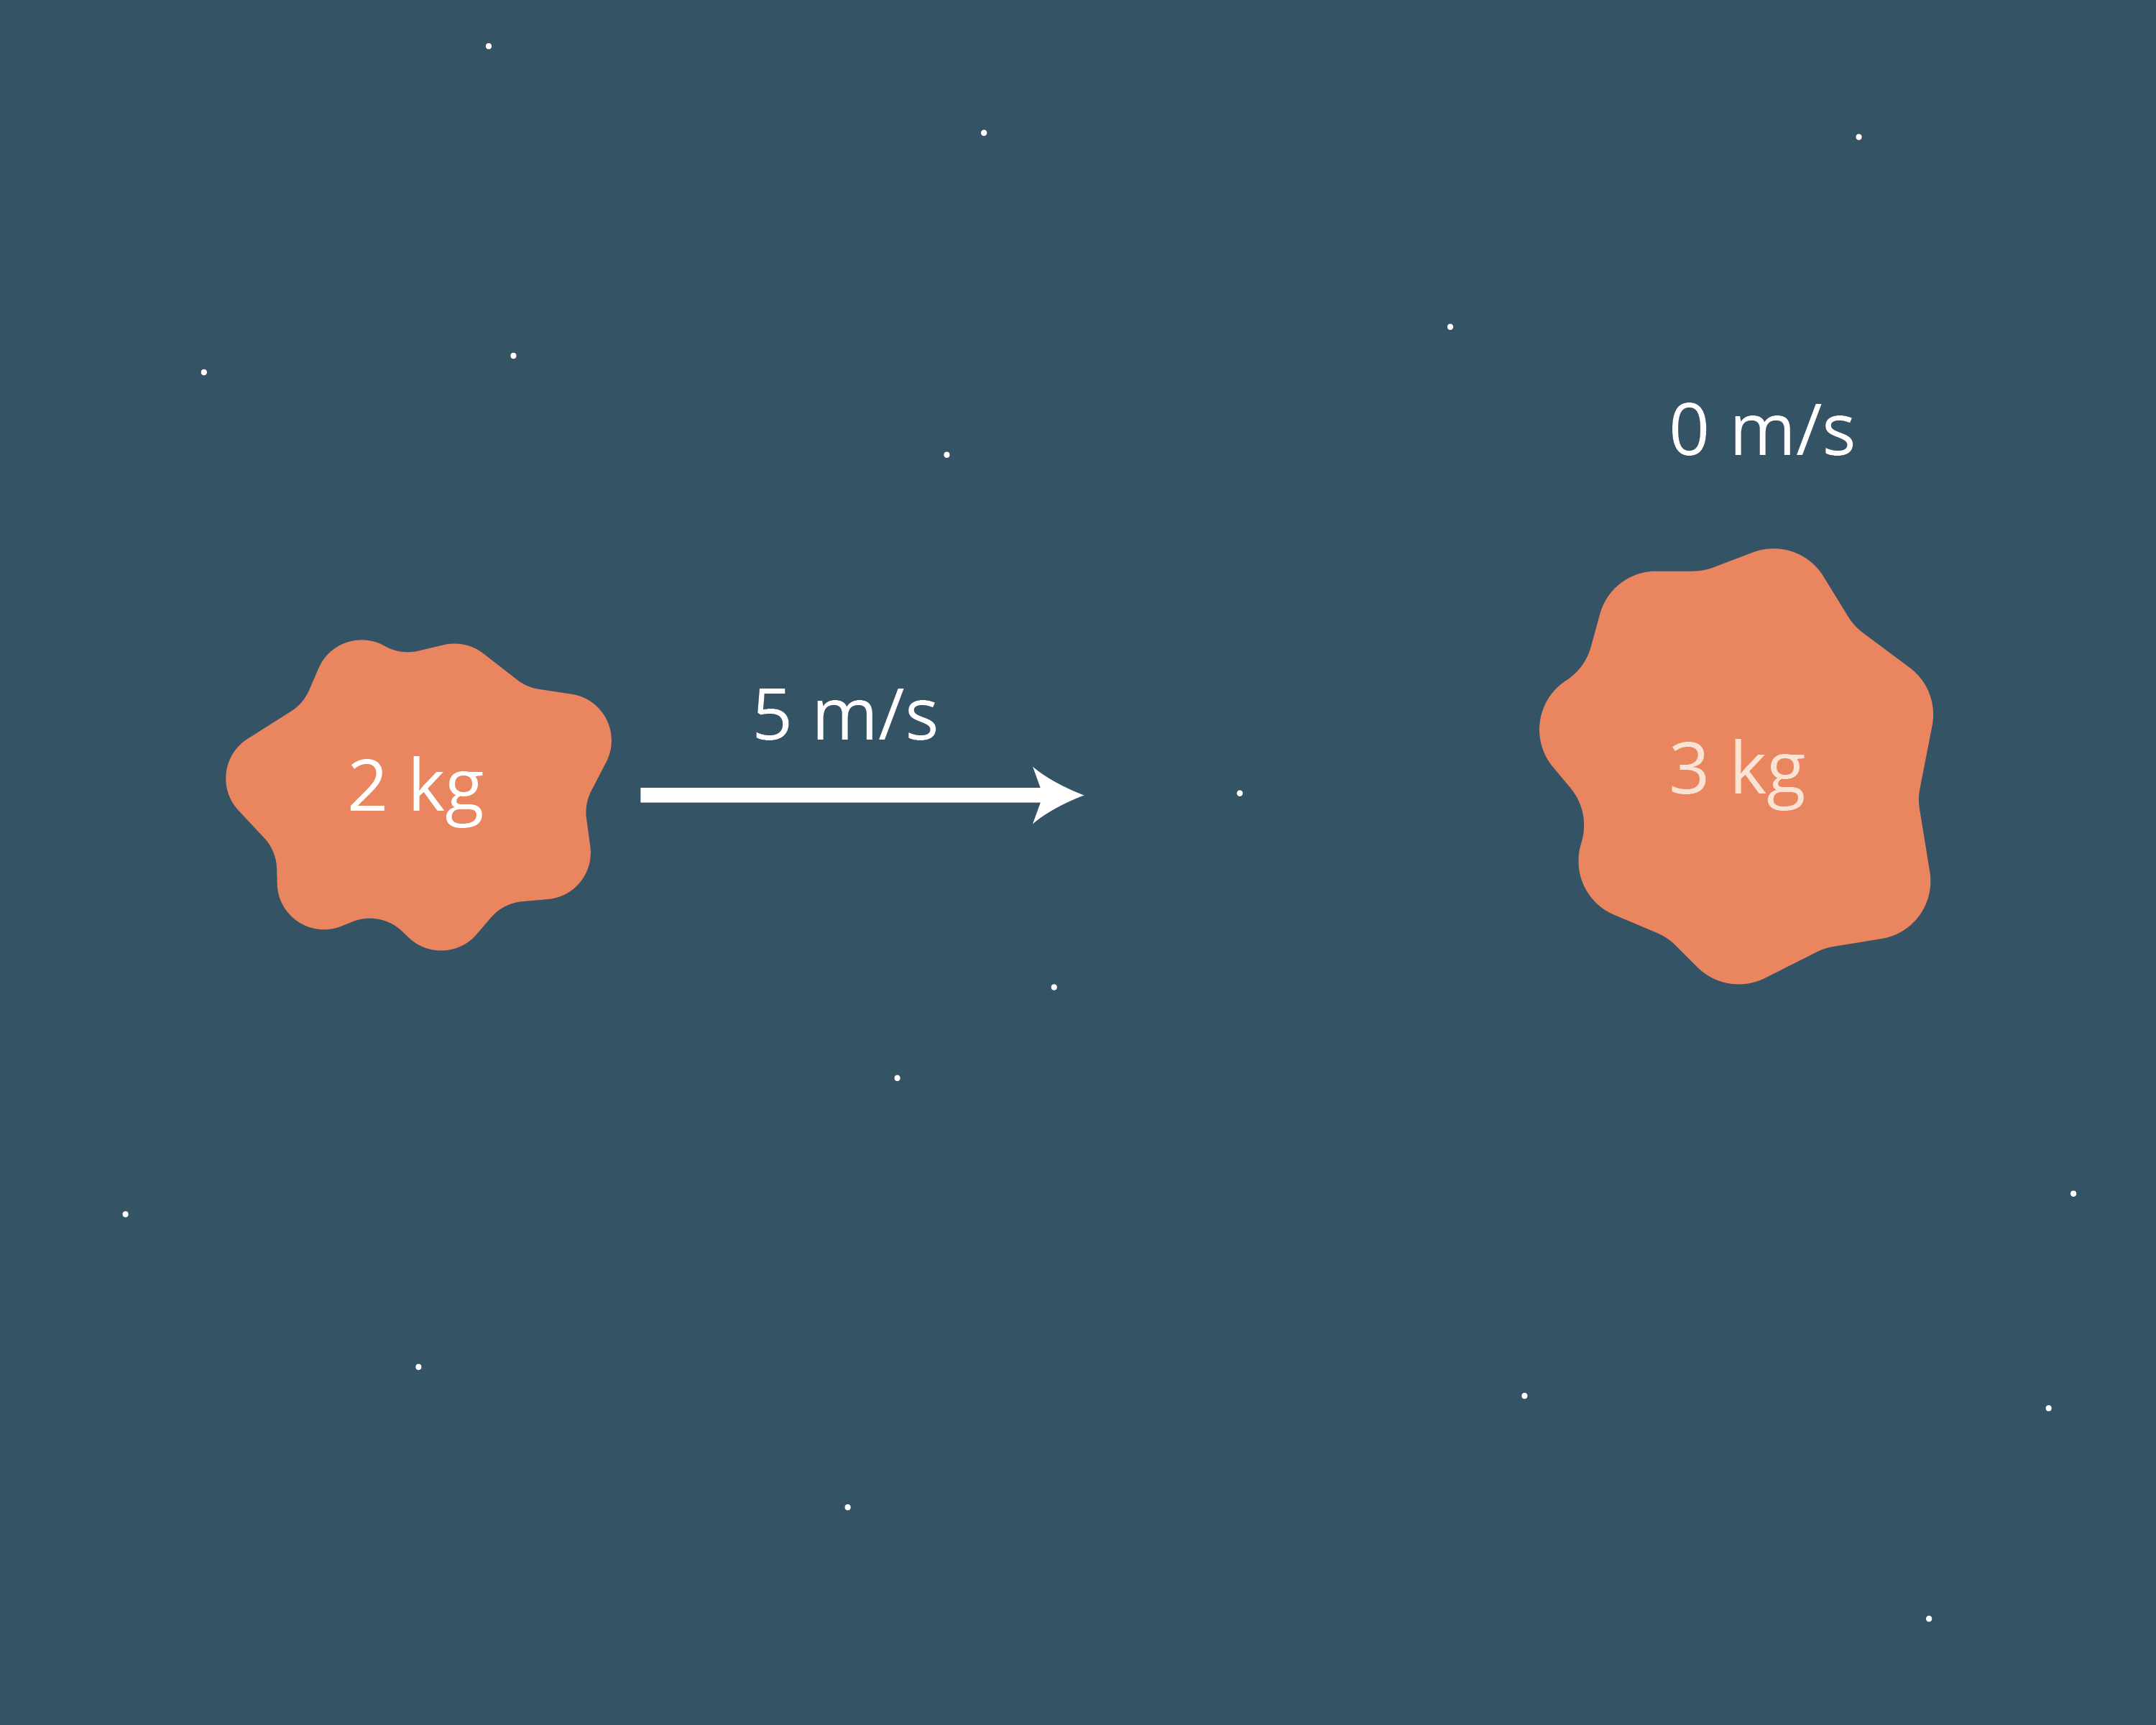
\includegraphics[width=0.4\textwidth]{putty1.png}
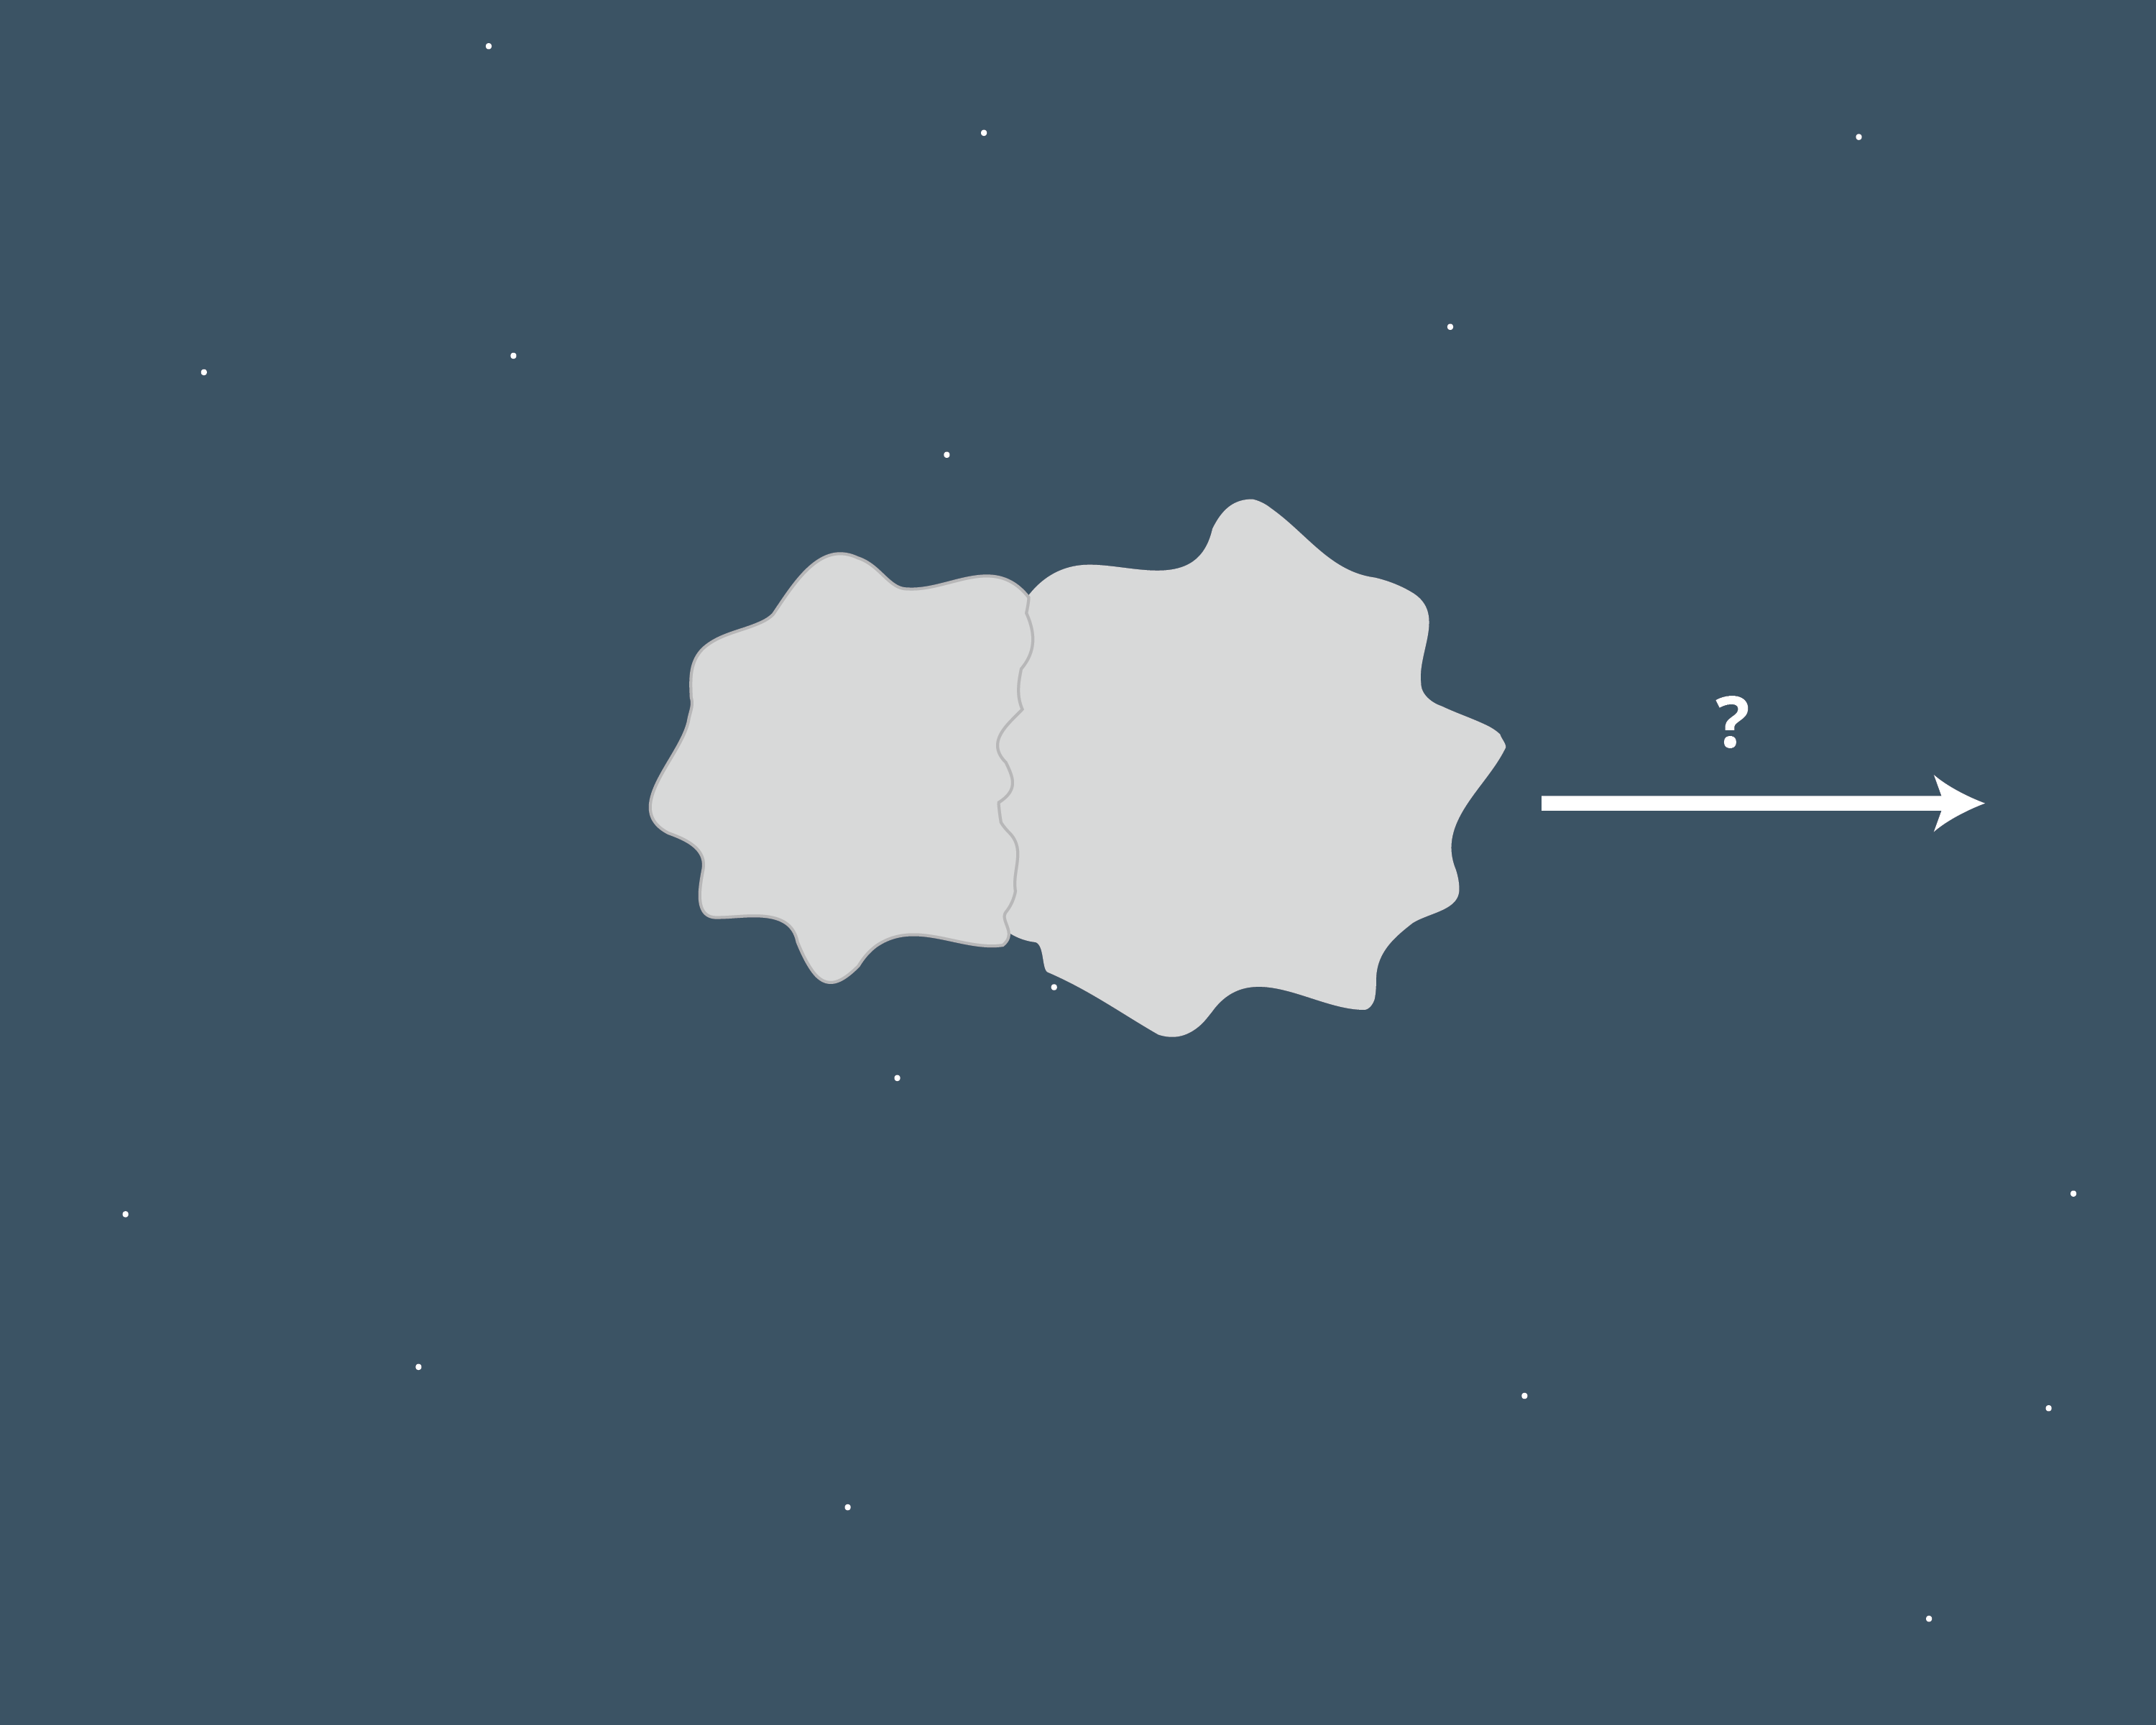
\includegraphics[width=0.4\textwidth]{putty2.png}


Every object has \newterm{momentum}.  The momentum is a vector
quantity: It points in the direction that the object is moving and has
a magnitude equal to its mass times its speed.

Given a set of objects that are interacting, we can sum all their
momentum vectors to get the total momentum.  In such a set, the total
momentum will stay constant.

So, in our example, one object has a momentum vector of magnitude of
10 kg m/s, the other has a momentum of magnitude 0.  Once they have
merged, they have a combined mass of 5 kg.  Thus, the velocity vector
must have magnitude 2 m/s and pointing in the same direction that the
first mass was moving.

\begin{Exercise}[title={Cars on Ice}, label=cars_on_ice]
A car weighing 1000 kg is going north at 12 m/s.  Another car weighing
1500 kg is going east at 16 m/s.  They both hit a patch of ice (with
zero friction) and collide.  Steel is bent and the two objects become
one.  How what is the velocity vector (direction and magnitude) of the
new object sliding across the ice?
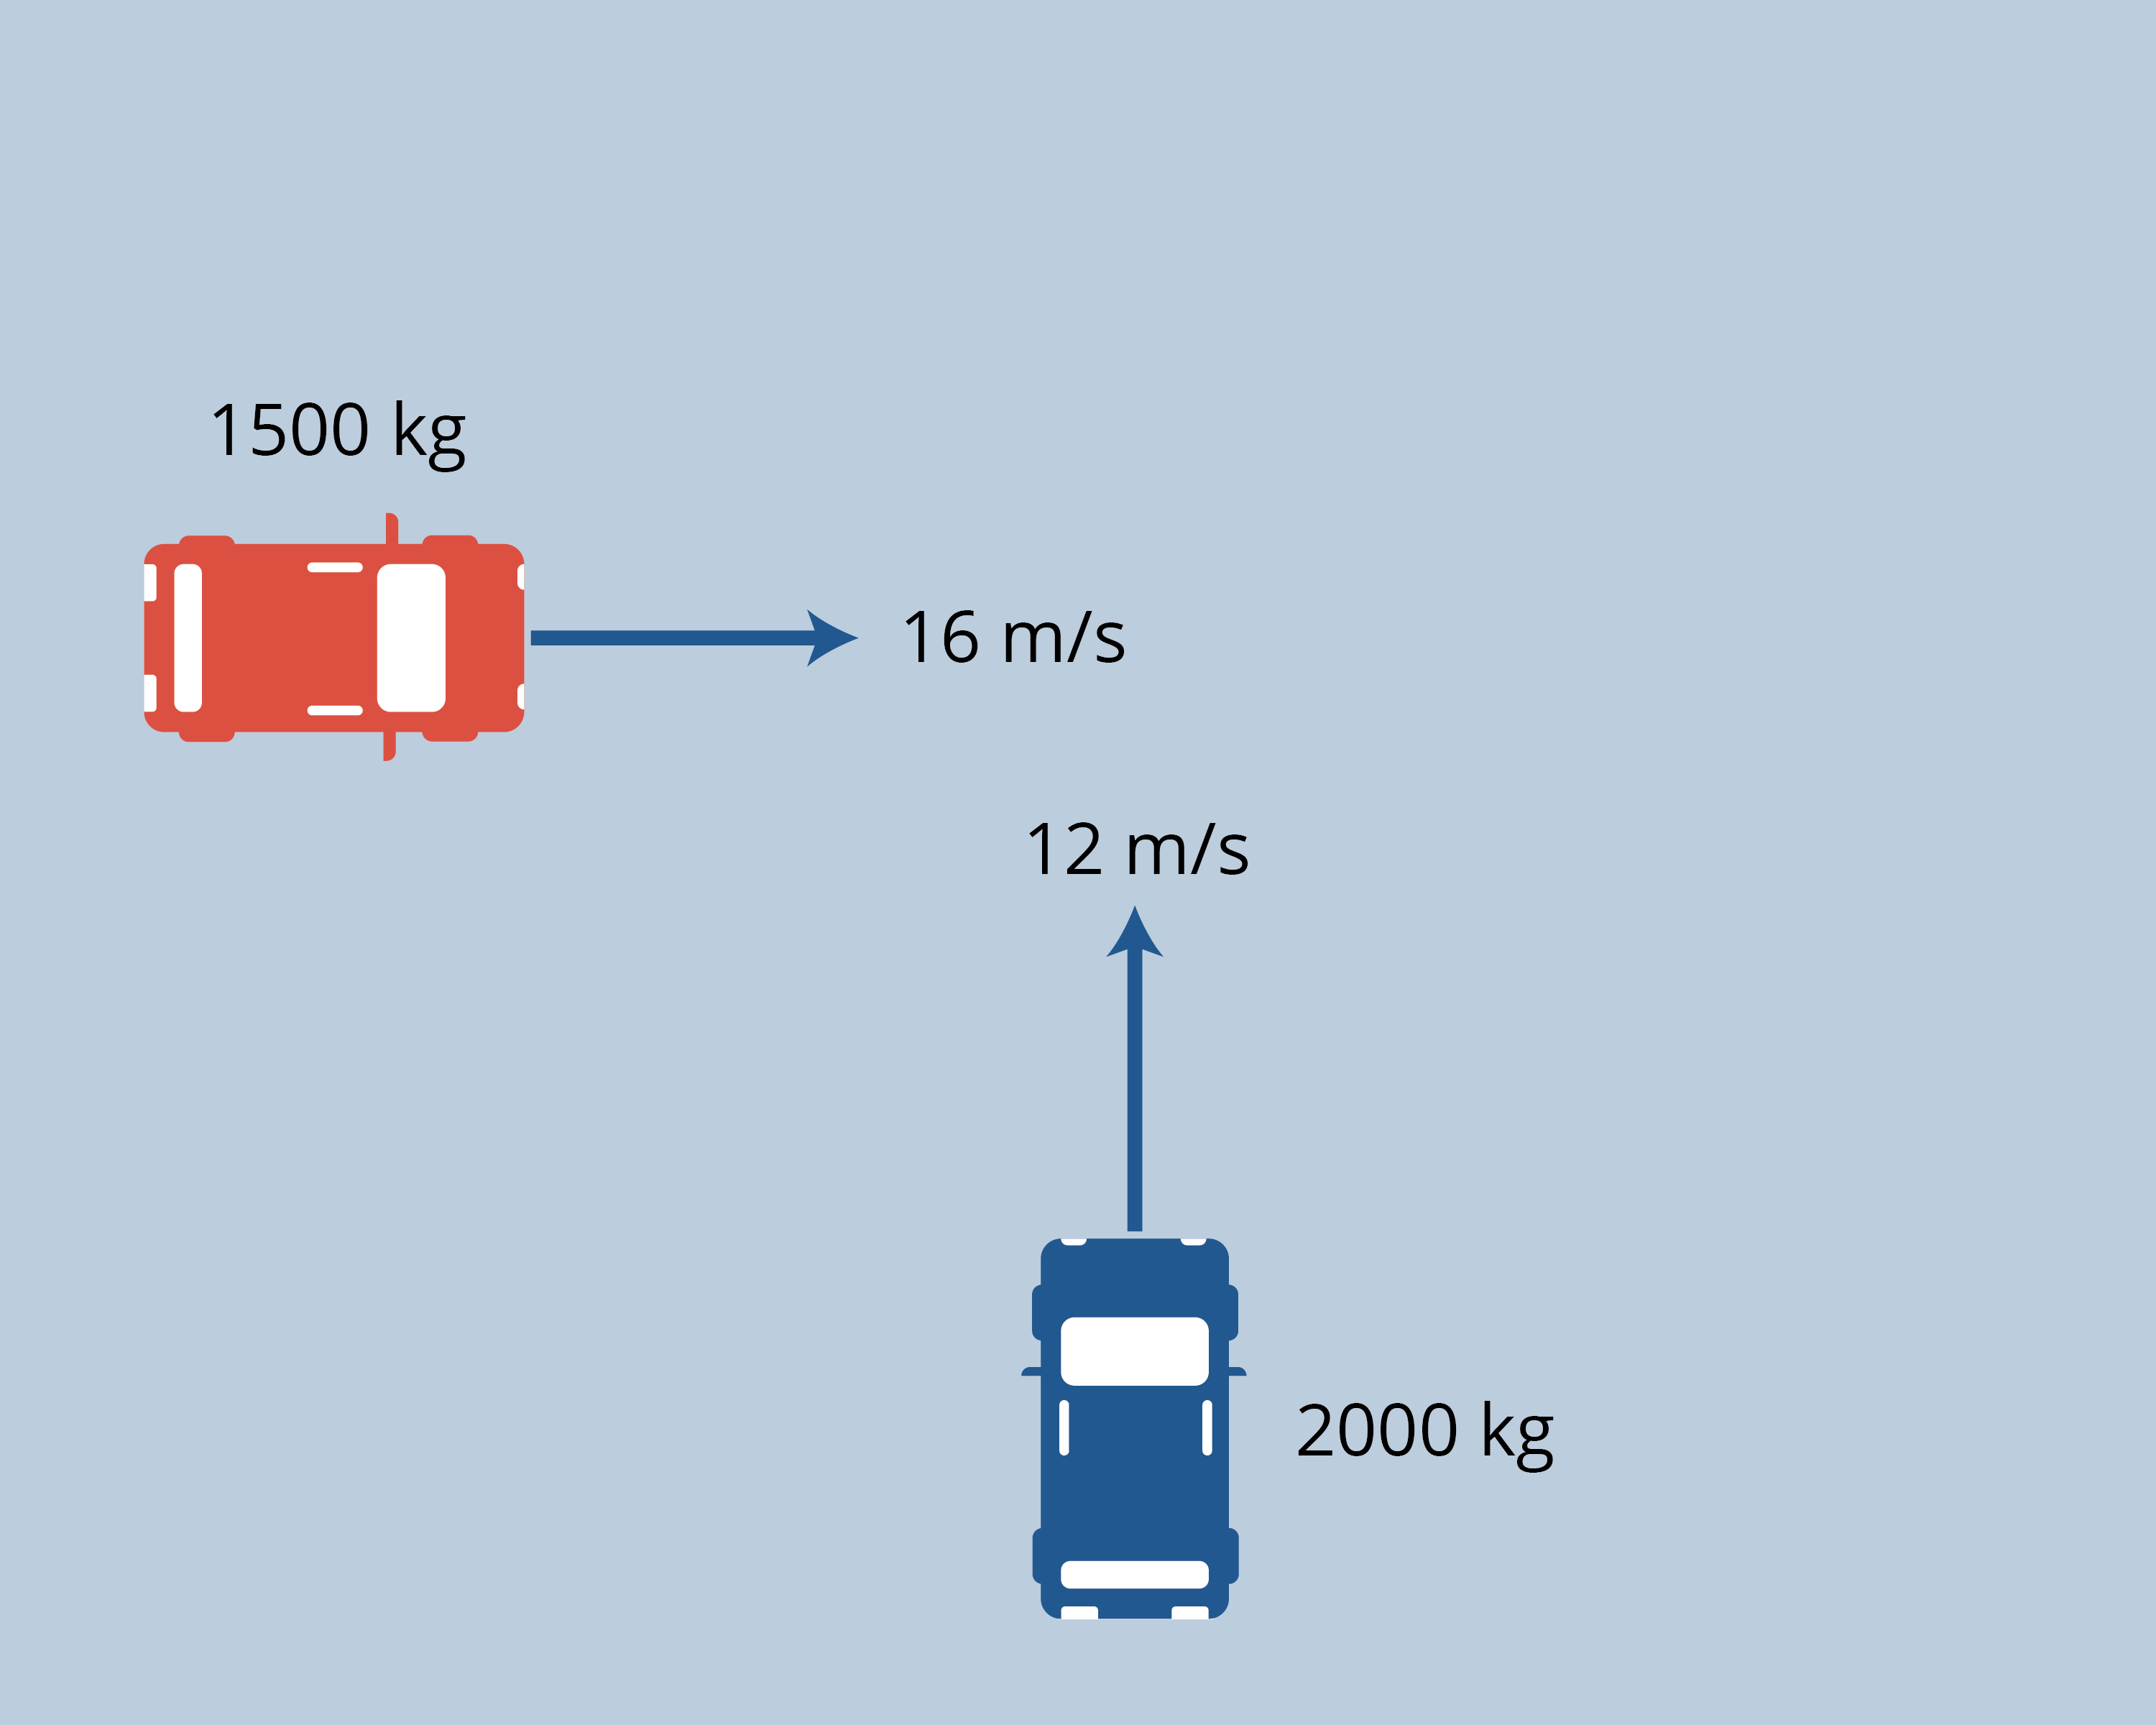
\includegraphics[width=0.4\textwidth]{icecar.png}
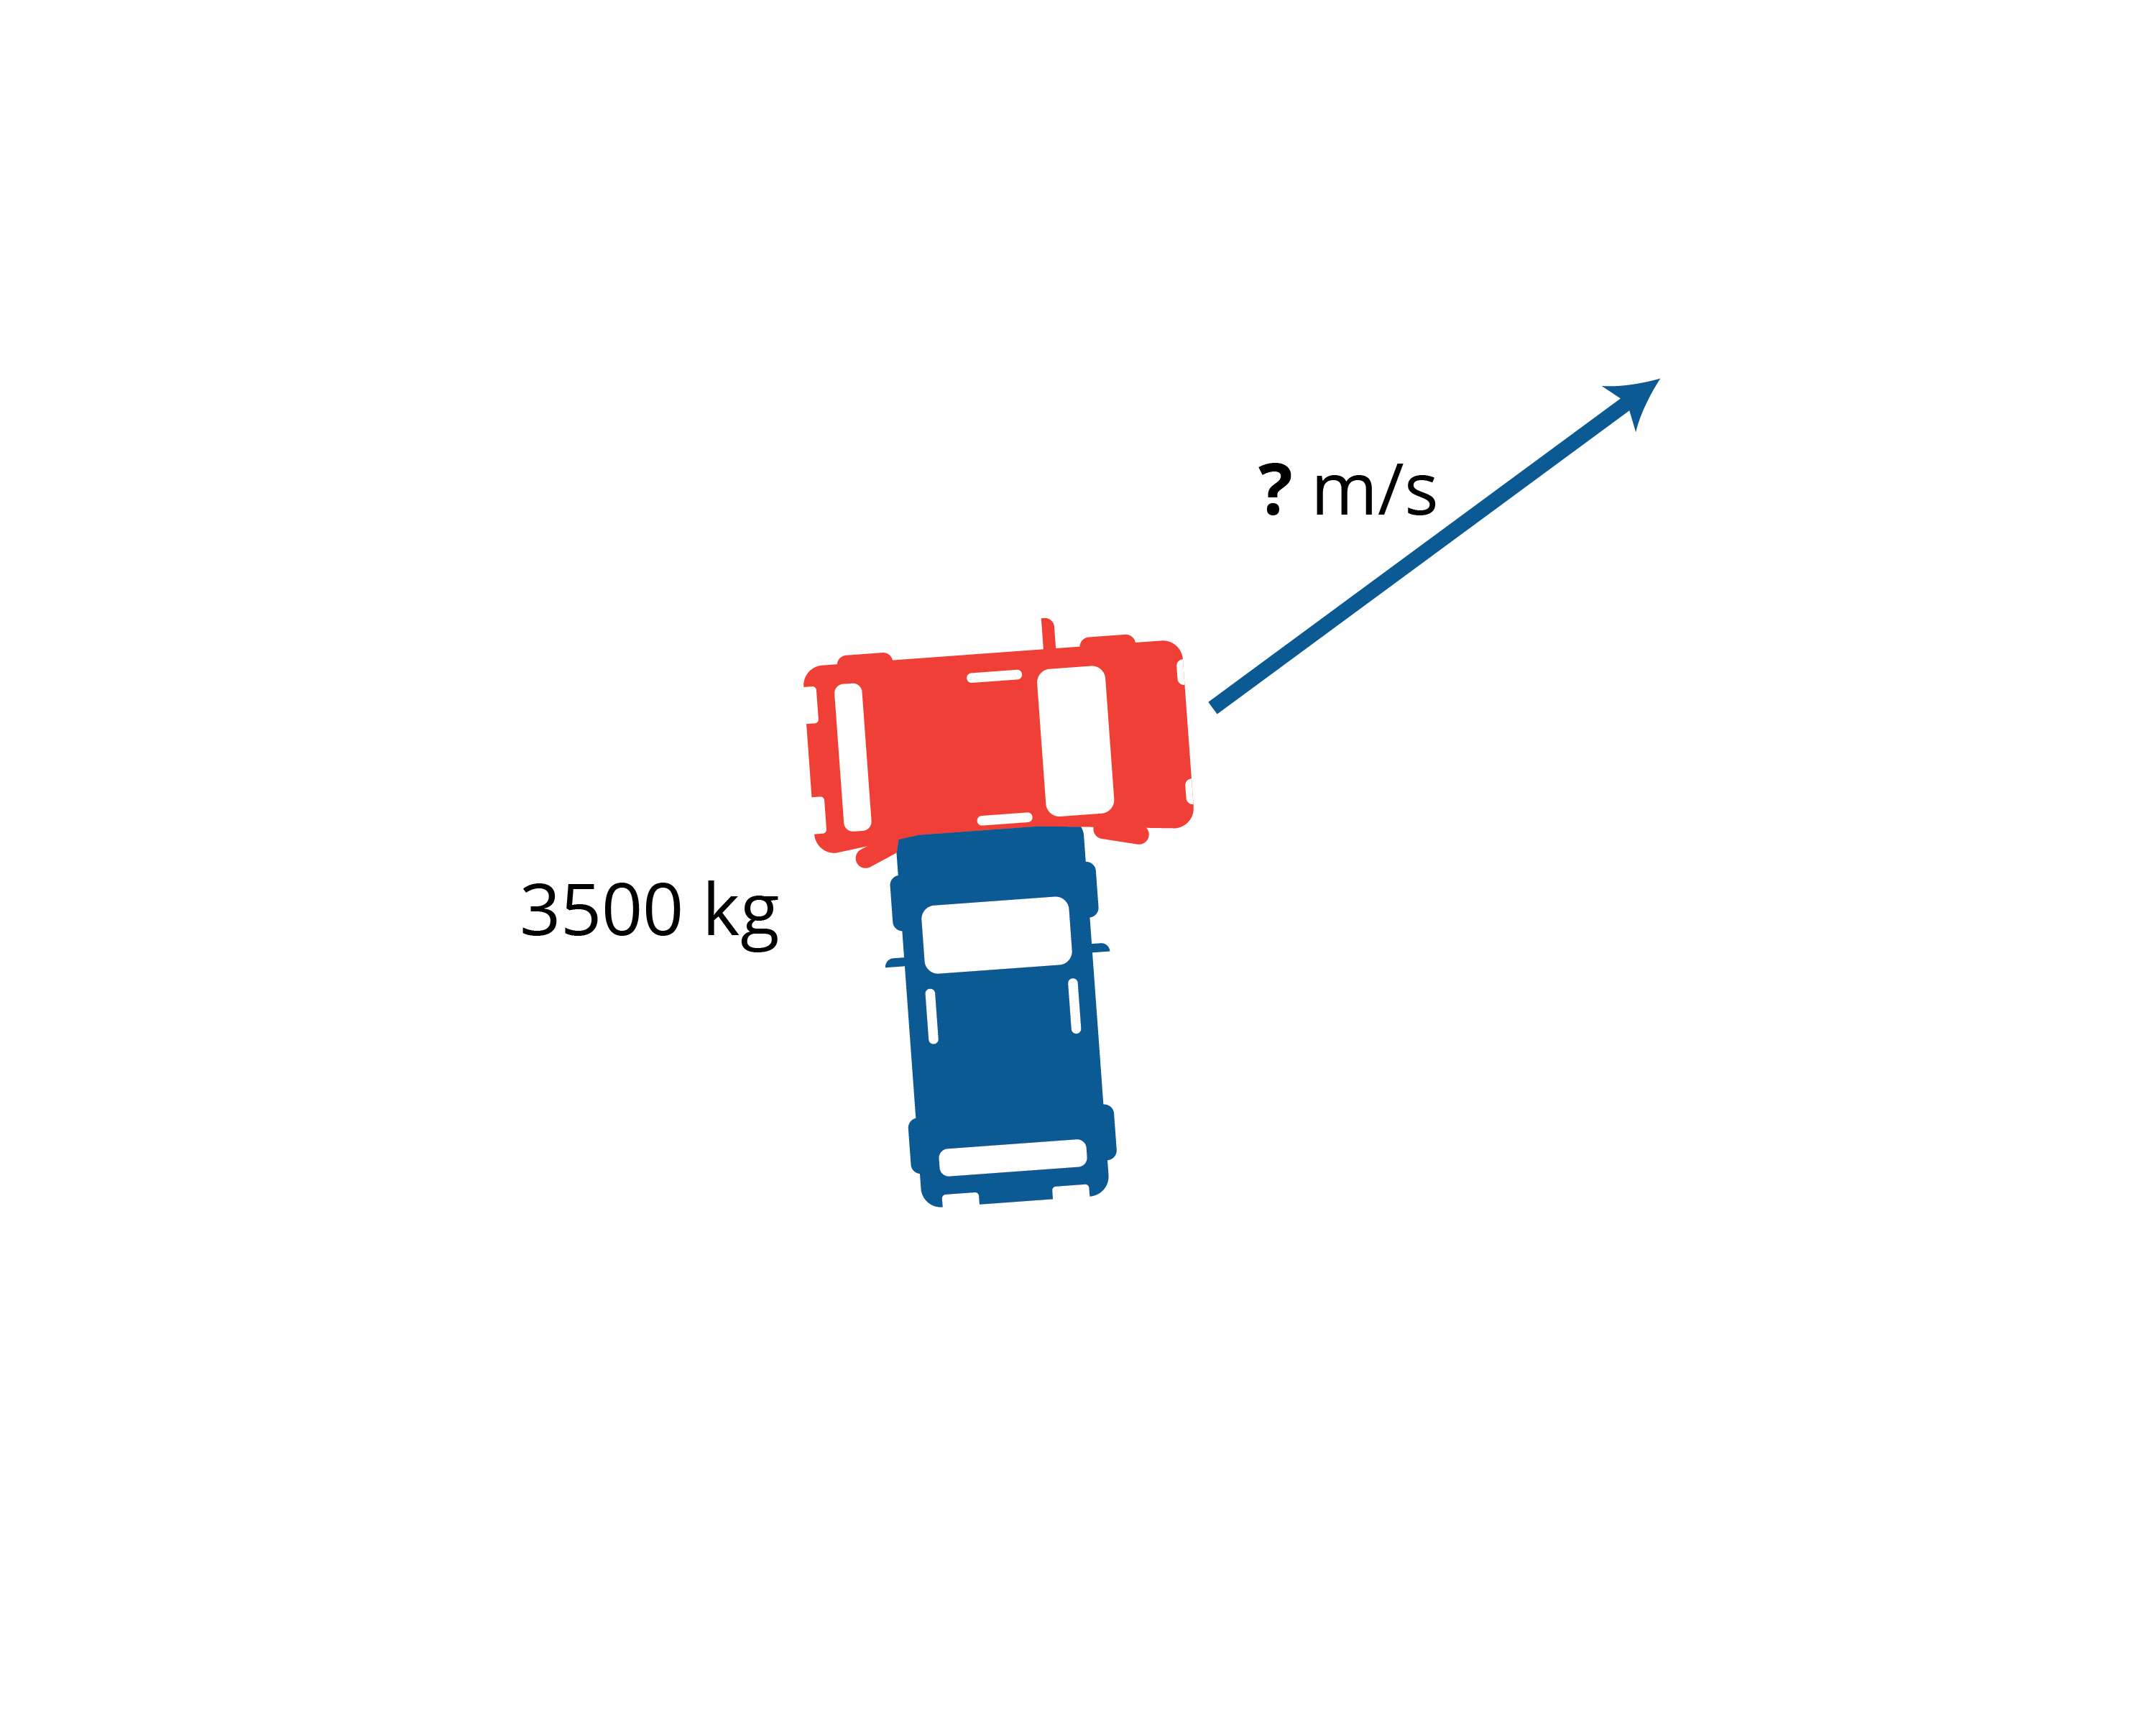
\includegraphics[width=0.4\textwidth]{icecar2.png}

\end{Exercise}
\begin{Answer}[ref=cars_on_ice]
  The momentum of the first car is 12,000 kg m/s in the north direction.

  The momentum of the second car is 24,000 kg m/s in the east direction.

  The new object will be moving northeast. What angle is the angle compared with the east?

  $$\theta = \arctan{\frac{12,000}{24,000}} \approx 0.4636 \text{ radians } \approx 26.565\text{ degrees north of east}$$

  The magnitude of the momentum of the new object is $\sqrt{12,000^2 + 24,000^2} \approx 26,833\text{ kg m/s}$

  Its new mass is 2,5000 kg.  So the speed will be $26,833/2,500 = 10.73$ m/s.
\end{Answer}


Notice that kinetic energy ($1/2 m v^2$) is \emph{not} conserved
here.  Before the collision, the moving putty block has $(1/2)(2)(5^2) = 25$
joules of kinetic energy.  Afterward, the big block has $(1/2)(5)(2^2)
= 10$ joules of kinetic energy.  What happened to the energy that was
lost? It was used up deforming the putty.

What if the blocks were marble instead of putty?  Then there would be
very little deforming, so kinetic energy \emph{and} momentum would be
conserved. The two blocks would end up having different velocity
vectors.

Let's assume for a moment that they strike each other straight on, so
there is motion in only one direction, both before and after the
collision.  Can we solve for the speeds of the first block ($v_1$) and
the second block ($v_2$)?

We end up with two equations. Conservation of momentum says:

$$2 v_1 + 3 v_2 = 10$$

Conservation of kinetic energy says:

$$(1/2)(2)(v_1^2) + (1/2)(3)(v_2^2) = 25$$

Using the first equation, we can solve for $v_1$ in terms of $v_2$:

$$v_1 = \frac{10 - 3 v_2}{2}$$

Substituting this into the second equation, we get:

$$\left(\frac{10 - 3 v_2}{2}\right)^2 + \frac{3 v_2^2}{2} = 25$$

Simplifying, we get:

$$v_2^2 - 4 v_2 + 0 = 0$$

This quadratic has two solutions: $v_2 = 0$ and $v_2 = 4$.  $v_2 = 0$
represents the situation before the collision.  Substituting in $v_2 = 4$:

$$v_1 = \frac{10 - 3(4)}{2} = -1$$

Thus, if the blocks are hard enough that kinetic energy is conserved,
after the collision, the smaller block will be heading in the opposite
direction at 1 m/s.  The larger block will be moving at 4 m/s in the
direction of the original motion.

\begin{Exercise}[title={Billiard Balls}, label=billiards]
  
A billiard ball weighing 0.4 kg and traveling at 3 m/s hits a billiard
ball (same weight) at rest. It strikes obliquely so that the ball at rest starts to
move at a 45 degree angle from the path of the ball that hit it.

Assuming all kinetic energy is conserved. How what is the velocity
vector of each ball after the collision?

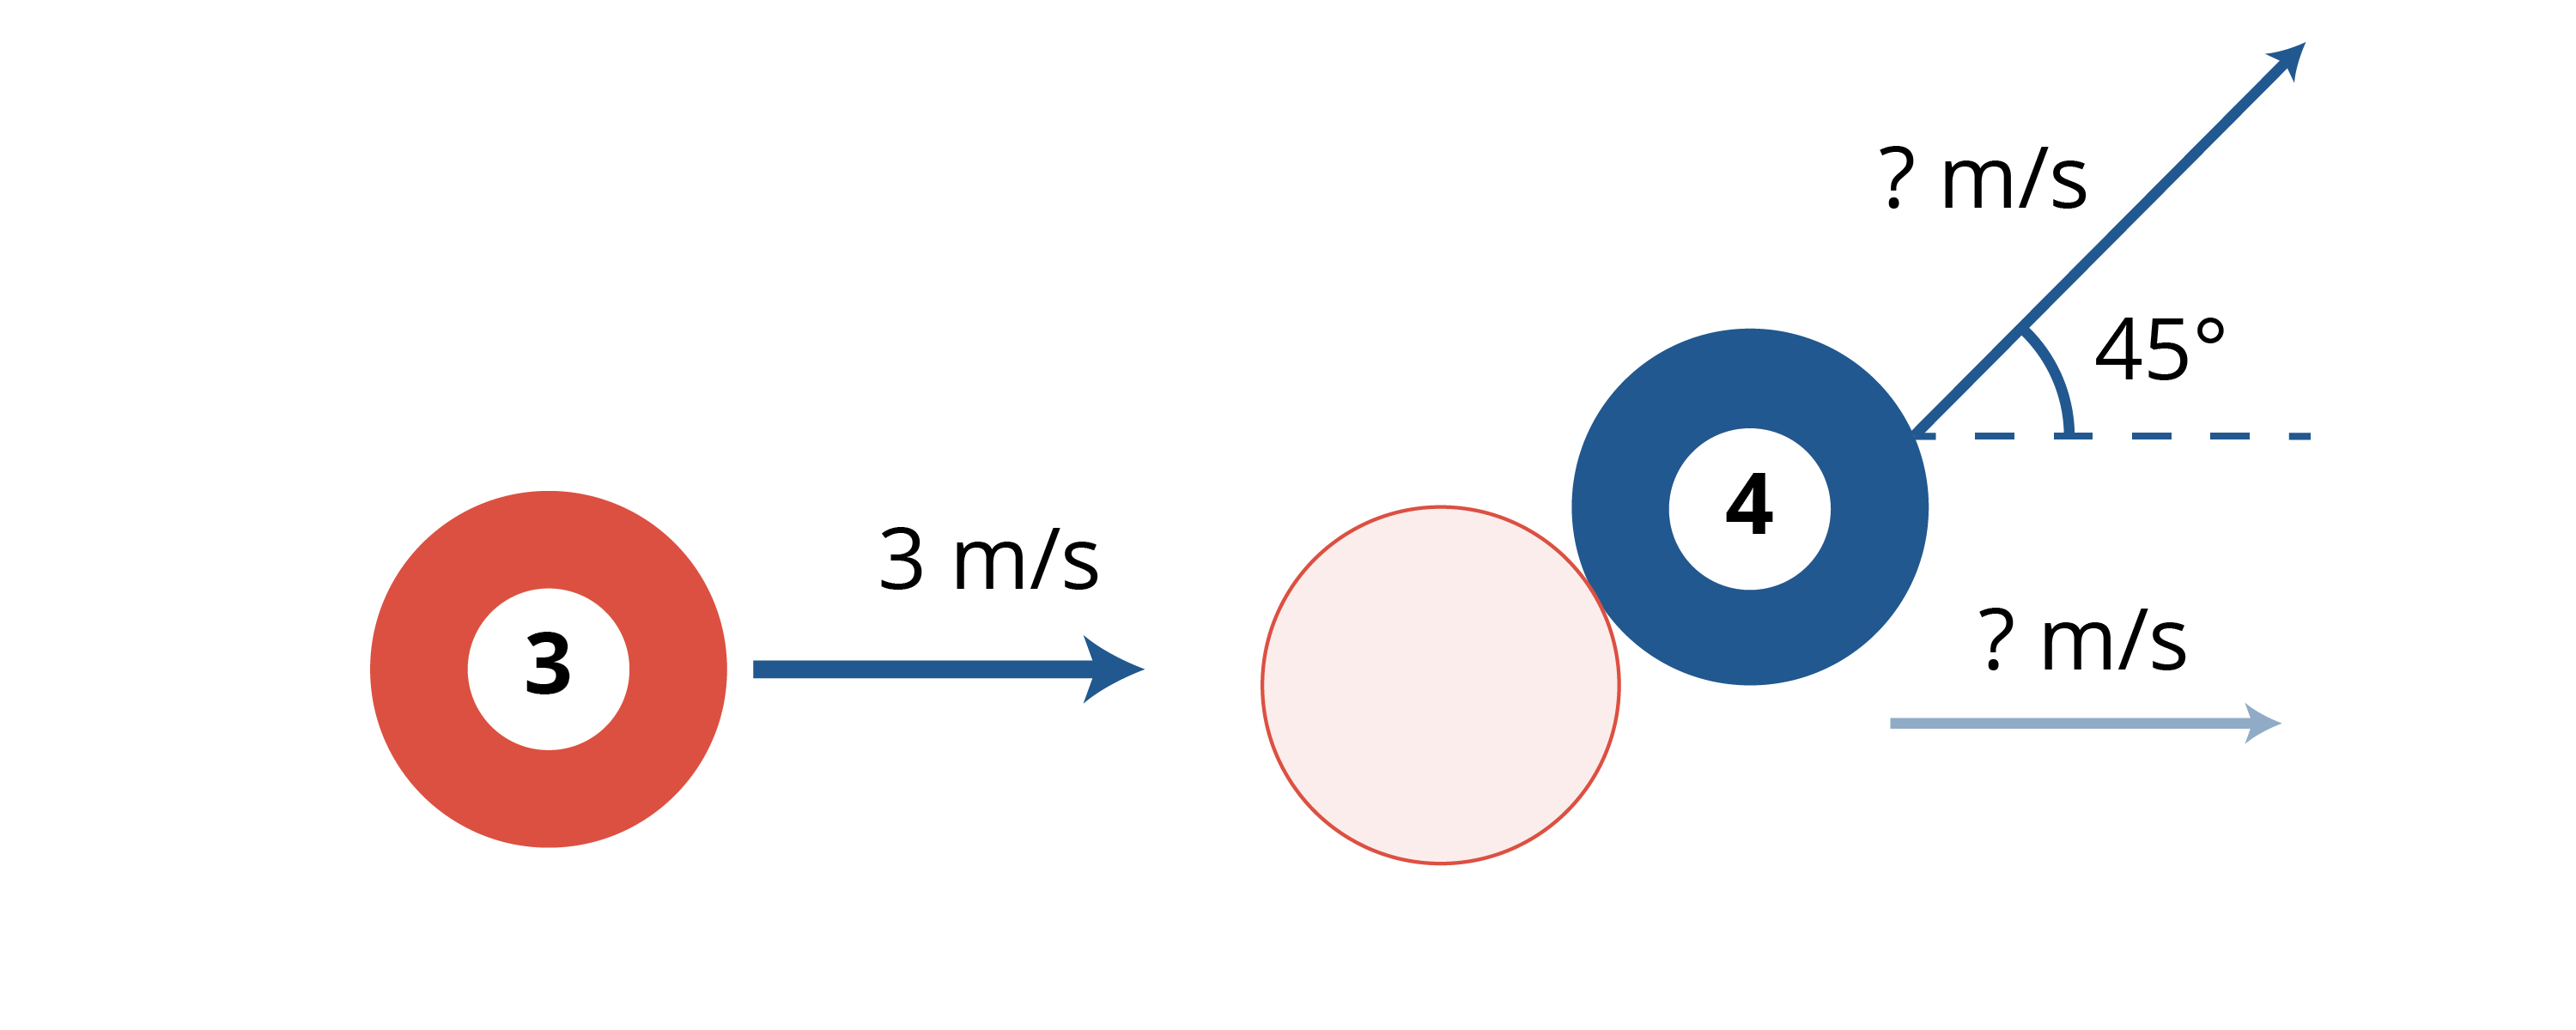
\includegraphics[width=1\textwidth]{poolball.png}

\end{Exercise}
\begin{Answer}[ref=billiards]

  The original forward momentum was 1.2 kg m/s.  The original kinetic energy is $(1/2)(0.4)(3^2)$ = 1.8 joules. 

  Let $s$ be the post-collision speed of the ball that had been at
  rest.  Let $x$ and $y$ be the forward and sideways speeds
  (post-collision) of the other ball. Conservation of kinetic energy says

  $$(1/2)(0.4)(s^2) + (1/2)(0.4)(x^2+y^2) = 1.8$$

  Forward momentum is conserved:

  $$0.4\frac{s}{\sqrt{2}} + 0.4 x = 1.2$$

  Which can be rewritten:

  $$x = 3 - \frac{s}{\sqrt{2}}$$
  
  Sideways momentum stays zero:

  $$(0.4)\frac{s}{\sqrt{2}} - 0.4 y = 0.0$$

  Which can be rewritten:

  $$y = \frac{s}{\sqrt{2}}$$

  Substituting into to the conservation of kinetic energy equation above:

  $$(1/2)(0.4)(s^2) + (1/2)(0.4)(\left(3 - \frac{s}{\sqrt{2}}\right)^2+\left(\frac{s}{\sqrt{2}}\right)^2 = 1.8$$

  Which can be rewritten:

  $$s^2 - \frac{3}{\sqrt{2}} s + 0 = 0$$

  There are two solutions to this quadratic: $s = 0$ (before collision) and $s = \frac{3}{\sqrt{2}}$. Thus,

  $$y = \frac{3}{2}$$

  and

  $$x = 3 - \frac{3}{2} = \frac{3}{2}$$

  So both balls careen off at $45^\circ$ angles at the exact same speed. 

  
\end{Answer}




\graphicspath{{../../Chapters/dot/en_US}}
\chapter{The Dot Product}
% Reference for diagrams:https://www.mathsisfun.com/algebra/vectors-dot-product.html

If you have two vectors $\textbf{u} = [u_1, u_2, \dots, u_n]$ and $\textbf{v} 
= [v_1, v_2,\dots, v_n]$, we define the \newterm{dot product} $\textbf{u} 
\cdot \textbf{v}$ as 
\begin{equation*}
     \textbf{u} \cdot \textbf{v} = (u_1 \times v_1) + (u_2 \times v_2) + \dots 
     + (u_n \times v_n)
\end{equation*} 
The output of the dot product is a \emph{scalar} quantity.


For example, 
\begin{equation*}
    [2,4, -3] \cdot [5, -1, 1] = 2 \times 5 + 4 \times -1 + -3 \times 1 = 3
\end{equation*}\index{dot product}

This may not seem like a very powerful idea, but dot products are 
\emph{incredibly} useful. The enormous GPUs (Graphics Processing Units) that 
let video games render scenes so quickly? They primarily function by computing 
huge numbers of dot products at mind-boggling speeds. 

\begin{Exercise}[title={Basic dot products}, label=dot_products]
    Compute the dot product of each pair of vectors:
    \begin{itemize}
        \item $[1, 2, 3]$, $[4, 5, -6]$
        \item $[\pi, 2\pi]$, $[2, -1]$
        \item $[0,0,0,0]$, $[10,10,10,10]$
    \end{itemize}
\end{Exercise}
\begin{Answer}[ref=dot_products]
        \begin{itemize}
            \item $[1, 2, 3] \cdot [4, 5, -6] = 4 + 10 - 18 = -4$
            \item $[\pi, 2\pi] \cdot [2, -1] = 2\pi - 2\pi = 0$
            \item $[0,0,0,0] \cdot [10,10,10,10] = 0 + 0 + 0 + 0 = 0$ 
        \end{itemize}
\end{Answer}

\section{Properties of the dot product}

Sometimes we need an easy way to say ``The vector of appropriate length is 
filled with zeros.'' We use the notation $\vec{0}$ to represent this. Then, 
for any vector $\textbf{v}$, this is true:

$$\textbf{v} \cdot \vec{0} = 0$$

The dot product is commutative:

$$\textbf{v} \cdot \textbf{u} = \textbf{u} \cdot \textbf{v}$$

The dot product of a vector with itself is its magnitude squared:

$$ \textbf{v} \cdot \textbf{v} = |\textbf{v}|^2 $$

If you have a scalar $a$, then:

    $$(\textbf{v}) \cdot (a \textbf{u}) = a (\textbf{v} \cdot \textbf{u})$$

So, if $\textbf{v}$ and $\textbf{w}$ are vectors that go in the same direction,

    $$\textbf{v} \cdot \textbf{w} = |\textbf{v}| |\textbf{w}|$$

If $\textbf{v}$ and $\textbf{w}$ are vectors that go in opposite directions,

    $$\textbf{v} \cdot \textbf{w} = -|\textbf{v}| |\textbf{w}|$$
    
If $\textbf{v}$ and $\textbf{w}$ are vectors that are perpendicular to each 
other, their dot product is zero:

  $$ \textbf{v} \cdot \textbf{w} = 0 $$

\section{Cosines and dot products}

Furthermore, dot products' interaction with cosine makes them even more useful 
is what makes them so useful: 
If you have two vectors $\textbf{v}$ and $\textbf{u}$,

$$\textbf{v} \cdot \textbf{u} = |\textbf{v}| |\textbf{u}| \cos \theta$$

where $\theta$ is the angle between them.

So, for example, if two vectors $\textbf{v}$ and $\textbf{u}$ are 
perpendicular, the angle between them is $\pi/2$. The cosine of $\pi/2$ is 0. 
The dot product of any two perpendicular vectors is always 0. In fact, if the 
dot product of two non-zero vectors is 0, the vectors \textit{must be} 
perpendicular (see figure \ref{fig:perpendicular} for an example of 
perpendicular 2-dimensional vectors). 

\begin{figure}[htbp]
    \centering
    \begin{tikzpicture}
        \begin{axis}[xmin = -2, xmax = 5, ymin = 0, ymax = 5, 
        axis lines = center]
            \draw[blue, thick, -latex] (0, 0) -- (-1, 4) 
            node[above, black, font = \scriptsize] {$\left[ -1, 4 \right]$};
            \draw[blue, thick, -latex] (0, 0) -- (4, 1) 
            node[above, black, font = \scriptsize] {$\left[ 4, 1 \right]$};
        \end{axis}
    \end{tikzpicture}
    \caption{The dot product of any two perpendicular vectors is zero.}
    \label{fig:perpendicular}
\end{figure}
% cosine is not introduced before here
If you have two non-zero vectors $\textbf{v}$ and $\textbf{u}$, you can always 
compute the angle between them:\index{vectors!angle between}

$$\theta = \arccos{ \left( \frac{\textbf{v} \cdot \textbf{u}}{|\textbf{v}| 
|\textbf{u}|} \right)}$$

Arccos is short for arccosine, or $\cos^-1$, and it is a function that is the 
inverse of cosine. Cosine takes an angle and gives back the scaled 
$x$-component of the angle. Arccosine takes the $x$-component of an angle and 
returns an angle with that $x$-component. However, there is a limit to what 
arccos can return. Let's look at cosine and its inverse, arccos (see figures 
\ref{fig:cosine} and \ref{fig:arccos}). 

\begin{figure}[htbp]
    \centering
        \begin{tikzpicture}
            \begin{axis}[xmin = -0.5, xmax = 7, ymin = -1.25, ymax = 1.25, 
            axis lines = center, xlabel = $x$, ylabel = $y$]
                \addplot[blue, thick, samples = 150, domain = -0.5:7] 
                {cos(deg(x))};
            \end{axis}
        \end{tikzpicture}
        \caption{Cosine is a function: there is exactly one output for every 
        input.}
    \label{fig:cosine}
\end{figure}

\begin{figure}[htbp]
    \centering
    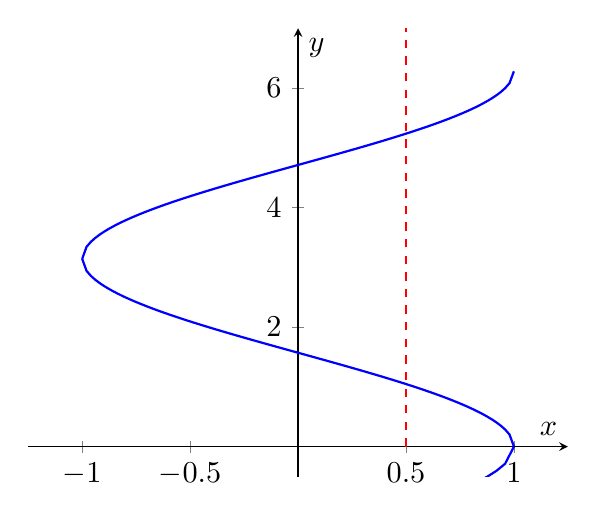
\begin{tikzpicture}
            \begin{axis}[xmin = -1.25, xmax = 1.25, ymin = -0.5, ymax = 7, 
            axis lines = center, xlabel = $x$, ylabel = $y$]
                \addplot[domain = -1:1, samples = 50, blue, thick]
                {-1*rad(acos(x))};
                \addplot[domain = -1:1, samples = 100, blue, thick]
                {rad(acos(x))};
                \addplot[domain = -1:1, samples = 100, blue, thick]
                {-1*rad(acos(x)) + 6.28319};
                \draw[red, thin, dashed] (0.5, 0) -- (0.5, 7);
            \end{axis}
        \end{tikzpicture}
    \caption{Arccos is not a function: there are many angles with the same 
    $x$-component. Notice that one input value has many output values (see the 
    red dashed line).}
    \label{fig:arccos}
\end{figure}

When you use a calculator to evaluate arccos, the calculator automatically 
restricts the results to between $0$ and $\pi$. Let's look at an example of 
using the dot product to determine the angle between two vectors:

\textbf{Example}: What is the angle between $\textbf{u} = \left[ \sqrt{3}, 1 
\right]$ and $\textbf{v} = \left[ 0, -1 \right]$?

\textbf{Solution}: We know that $\textbf{u} \cdot \textbf{v} = \left| 
\textbf{u} \right| \left| \textbf{v} \right| \cos{\theta}$. Therefore, we also 
know that:
$$\cos{\theta} = \frac{\textbf{u} \cdot \textbf{v}}{\left| \textbf{u} \right| 
\left| \textbf{v} \right|}$$

First, let's compute the dot product:
$$\textbf{u} \cdot \textbf{v} = \sqrt{3} \cdot 0 + 1 \cdot -1 = -1$$

And therefore:
$$\cos{\theta} = \frac{-1}{\left| \textbf{u} \right| \left| \textbf{v} 
\right|}$$

Now, let's find the magnitudes of both vectors:
$$\left| \textbf{u} \right| = \sqrt{\left( \sqrt{3} \right)^2 + \left( 1 
\right)^2} = 2$$
$$\left| \textbf{v} \right| = \sqrt{\left( 0 \right)^2 + \left( -1 \right)^2} 
= 1$$

Substituting for the magnitudes, we find that:
$$\cos{\theta} = \frac{-1}{2 \cdot 1} = \frac{-1}{2}$$

To solve for $\theta$, we take the $\arccos$ of both sides:
$$\arccos{ \left( \cos{\theta} \right)} = \theta = \arccos{ \frac{-1}{2} }$$

What angles have a cosine of $-1 / 2$? We know that $2\pi / 3$, $4 \pi / 3$, 
$8 \pi / 3$, etc., all have a cosine of $-1 / 2$. Because the range of 
$\arccos$ is restricted to between $0$ and $\pi$, our result is:
$$\theta = \arccos{ \frac{-1}{2}} = \frac{2\pi}{3}$$.

Therefore, the angle between \textbf{u} and \textbf{v} is $2\pi / 3$ (or $120^{
\circ}$). 

\begin{Exercise}[title={Using dot products}, label=cos_dot_products]
    What is the angle between these each pair of vectors:
    \begin{itemize}
        \item $[1, 0]$, $[0, 1]$
        \item $[3,4]$, $[4,3]$
        \item $[ 2, -1, 2 ]$, $[-1, 2, -2 ]$
        \item $[-5, 0, -1]$, $[2, 3, -4]$
    \end{itemize}
\end{Exercise}
\begin{Answer}[ref=cos_dot_products]
        \begin{itemize}
            \item $[1,0] \cdot [0,1] = 0$.  The angle must be $\pi/2$.
            \item $[3,4] \cdot [4, 3] = 24$. $|[3,4]| |[4,3]| \cos(\theta) = 24$. 
            $\cos(\theta) = \frac{24}{(5)(5)}$. $\theta = \arccos(\frac{24}{25}) 
            \approx 0.284 \text{ radians}$.
            \item $[2, -1, 2] \cdot [-1, 2, -2] = 4 - 2 - 4 = -2$. $|[2, -1, 2]| = \sqrt{4 + 1 + 4} = \sqrt{9} = 3$. $|[-1, 2, -2]| = \sqrt{1 + 4 + 4} = \sqrt{9} = 3$. $3(3) \cos{\theta} = -2$. $\theta = \arccos{ (-2 / 9)} \approx 1.795 \text{ radians}$.
            \item $[ -5, 0, -1] \cdot [2, 3, -4] = -10 + 0 + 4 = -6$. $|[-5, 0, 1]| = \sqrt{25 + 0 + 1} = \sqrt{26}$. $|[2, 3, -4]| = \sqrt{4 + 9 + 16} = \sqrt{29}$. $\sqrt{26} (\sqrt{29}) \cos{\theta} = -6$. $\theta = \arccos{(\frac{-6}{\sqrt{26}\sqrt{29}})} \approx 1.791 \text{ radians}$.
        \end{itemize}
\end{Answer}

\section{Dot products in Python}

NumPy will let you do dot products using the the symbol @.  Open \filename{first\_vectors.py} 
and add the following to the end of the script:

\begin{Verbatim}
    # Take the dot product
    d = v @ u
    print("v @ u =", d)
    
    # Get the angle between the vectors
    a = np.arccos(d / (mv * mu))
    print(f"The angle between u and v is {a * 180 / np.pi:.2f} degrees")    
\end{Verbatim}

When you run it you should get:
\begin{Verbatim}
v @ u = 4
The angle between u and v is 78.55 degrees
\end{Verbatim}

\section{Work and Power}
%diagram here
Earlier, we mentioned that mechanical work is the product of the 
force you apply to something and the amount it moves. For example, if you 
push a train with a force of 10 newtons as it moves 5 meters, you have done 50 joules of work.

What if you try to push the train sideways? It moves down the track 5 meters, 
but you push it as if you were trying to derail it --- perpendicular to its motion.  
You have done no work, because the train didn't move at all in the direction you were pushing.

% 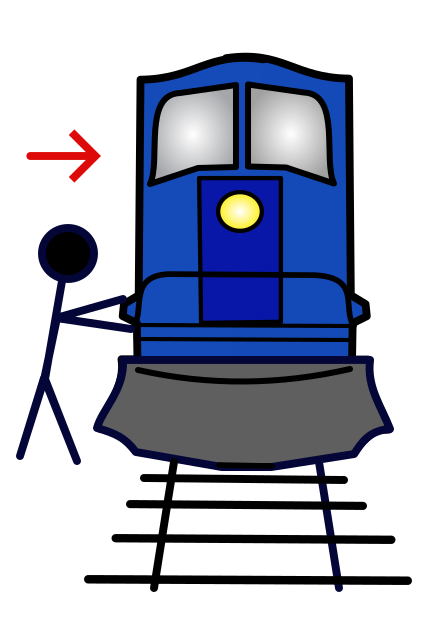
\includegraphics[width=0.8\textwidth]{train.png}


Now that you know about dot products: The work you do is the dot
product of the force vector you apply and the displacement vector of the train. (The displacement
vector is the vector that tells how the train moved while you pushed it.) \index{work}

Similarly, we mentioned that power is the product of the force you apply and the velocity of the
mass you are applying it to. It is actually the dot product of the force vector and the velocity vector.\index{power}

For example, if you are pushing a sled with a force of 10 newtons and it is moving 2 meters per second, 
but your push is 20 degrees off, you aren't transferring 20 watts of power to the sled.  
You are transferring $10 \times 2 \times \cos(20 \text{ degrees}) \approx 18.8$ watts of power.
%add ramps and sin

\graphicspath{{../../Chapters/functions/en_US}}
\chapter{Functions and Their Graphs}

Functions are a major part of science, engineering, and math. You can think of a function as a machine: you put something into the
machine, it processes it, and out comes something else: a product. Just as we
often use the variable $x$ to stand in for a number, we often use the
variable $f$ to stand in for a function. $f(x)$ is said as ``f of x``.
% One of my teachers told me half of understanding math is understanding mathmaticions are just lazy, maybe a good add in somewhere

For example, we might ask, ``Let the function $f$ be defined like this:

\begin{equation*}
f(x) = -5x^2 + 12x + 2
\end{equation*}

What is the value of $f(3)$, said as ``f of 3``?

You would run the number 3 through ``the machine'': $-5(3^2) + 12(3) + 2 = -7$. The answer would be ``$f(3)$ is $7$''.

However, some functions are not defined for every possible input. For example:

\begin{equation*}
  f(x) = \frac{1}{x}
\end{equation*}

  This is defined for any $x$ except 0, because you can't divide 1 by 0. The set of values that a function can process is called its \textit{domain}, and resulting output values are called the range.
  It is important to note that functions have only one \emph{output} for each \emph{input}. However, multiple inputs can have the same output. 
  A relationship where one input can result in the more than one output is not a function, but a relation. This can be proven by the \hyperref[sec:vertical]{vertical line test}.
% some good images could be found here: https://www.ck12.org/book/ck-12-algebra-i-honors/section/3.1/ 

\begin{Exercise}[title={Domain of a function}, label=function_domain]

  Let the function $f$ be given by $f(x) = \sqrt{x - 3}$.  What is its domain?

\end{Exercise}
\begin{Answer}[ref=function_domain]
  You can only take the square root of nonnegative numbers, so the
  function is only defined when $x - 3 \geq 0$.  Thus, the domain is
  all real numbers greater than or equal to 3.
\end{Answer}

\section{Graphs of Functions}

If you have a function, $f$, its graph is the set of pairs $(x, y)$
such that $y = f(x)$.  We usually draw a picture of this set, called a \textit{graph}. 
The graph not only includes the picture, but also the values of x and y used to create it.

Here is the graph of the function $f(x) = -5x^2 + 12x + 2$:

\begin{tikzpicture}
    \begin{axis}[
        xmin=-1,xmax=3.5,
        ymin=-10,ymax=11,
        axis x line=middle,
        axis y line=middle,
        axis line style=<->,
        xlabel={$x$},
        ylabel={$y$},
        ]
        \addplot[no marks,sdkblue,<->] expression[domain=-0.7:3.05,samples=100]{(-5)*(x^2) + (12 * x) + 2}; 
    \end{axis}
\end{tikzpicture}

(Note that this is just part of the graph; it goes infinitely in both
directions. Remember your vectors!)

Here is the graph of the function $f(x) = \frac{1}{x}$:

\begin{tikzpicture}
    \begin{axis}[
        xmin=-7,xmax=7,
        ymin=-7,ymax=7,
        axis x line=middle,
        axis y line=middle,
        axis line style=<->,
        xlabel={$x$},
        ylabel={$y$},
        ]
        \addplot[no marks,sdkblue,<->] expression[domain=-6.5:-0.15,samples=100]{1/x}; 
        \addplot[no marks,sdkblue,<->] expression[domain=0.15:6.5,samples=100]{1/x}; 
    \end{axis}
\end{tikzpicture}
To draw a graph, take each x value (usually in increments of 1) and determine its corresponding y value. 
Then, plot those points on a graph, using the origin as the starting point. 
% do we assume students know how to graph?
\begin{Exercise}[title={Draw a graph}, label=draw_graph]

  Let the function $f$ be given by $f(x) = -3x + 3$. Sketch its graph.
% More space needed in exercise box
\end{Exercise}
\begin{Answer}[ref=draw_graph]

  The graph of this function is a line, its slope is -3, and it intersects the y axis at $(0, 3)$.

\begin{tikzpicture}
    \begin{axis}[
        xmin=-1,xmax=3,
        ymin=-7,ymax=7,
        xtick={1},
        ytick={3},
        axis x line=middle,
        axis y line=middle,
        axis line style=<->,
        xlabel={$x$},
        ylabel={$y$},
        ]
        \addplot[no marks,sdkblue,<->] expression[domain=-0.75:2.74,samples=100]{-3 * x + 3}; 
    \end{axis}
\end{tikzpicture}
  
  
\end{Answer}


\section{Can this be expressed as a function?}
\label{sec:vertical}

Note that not all sets can be expressed as graphs of functions.  For
example, here is the set of points $(x,y)$ such that $x^2 + y^2 = 9$:

\begin{tikzpicture}
    \begin{axis}[
        xmin=-3.5,xmax=3.5,
        ymin=-3.5,ymax=3.5,
        ytick={-3,-2,-1,0,1,2,3},
        axis x line=middle,
        axis y line=middle,
        axis line style=<->,
        xlabel={$x$},
        ylabel={$y$},
        ]
        \addplot[no marks,sdkblue] expression[domain=-3:3,samples=100]{sqrt(9 - x^2)}; 
        \addplot[no marks,sdkblue] expression[domain=-3:3,samples=100]{-1 * sqrt(9 - x^2)}; 
    \end{axis}
\end{tikzpicture}

This cannot be the graph of a function, because what would $f(0)$ be? 3
or -3?  This set fails what we call ``the vertical line test'': If any
vertical line contains more than one point from the set, it isn't the graph
of a function.  For example, the vertical line $x = 2$ would cross the graph twice:
\begin{center}
  
  \begin{tikzpicture}
    \begin{axis}[
      xmin=-3.5,xmax=3.5,
      ymin=-3.5,ymax=3.5,
      ytick={-3,-2,-1,0,1,2,3},
      axis x line=middle,
      axis y line=middle,
      axis line style=<->,
      xlabel={$x$},
      ylabel={$y$},
      ]
      \addplot[no marks,sdkblue] expression[domain=-3:3,samples=100]{sqrt(9 - x^2)}; 
      \addplot[no marks,sdkblue] expression[domain=-3:3,samples=100]{-1 * sqrt(9 - x^2)};
      \addplot [thick, dashed] coordinates {(2,-2.5)(2,2.5)};
      
    \end{axis}
    
  \end{tikzpicture}
\end{center}
%might be a good place to talk about even vs odd functions
\index{vertical line test}

\section{Inverses}

Some functions have inverse functions. If a function $f$ is a machine that turns
number $x$ into $y$, the inverse (usually denoted $f^{-1}$) is the machine that turns $y$ back
into $x$.

For example, let $f(x) = 5x + 1$. Its inverse is
$f^{-1}(x) = (x - 1)/5$. (Spot check it: $f(3) = 16$ and $f^{-1}(16) = 3$)

Does the function $f(x) = x^3$ have an inverse? Yes, $f^{-1}(x) =
\sqrt[3]{x}$. Let's plot the function (solid line) and its inverse (dashed):

\begin{tikzpicture}
    \begin{axis}[
        xmin=-3.5,xmax=3.5,
        ymin=-3.5,ymax=3.5,
        ytick={-3,-2,-1,0,1,2,3},
        axis x line=middle,
        axis y line=middle,
        axis line style=<->,
        xlabel={$x$},
        ylabel={$y$},
        ]
        \addplot[no marks,sdkblue] expression[domain=-3:3,samples=100]{x^3}; 
        \addplot[no marks,sdkblue,dashed] expression[domain=0:3,samples=100]{x^(1/3)}; 
        \addplot[no marks,sdkblue,dashed] expression[domain=-3:0,samples=100]{-1 * (-1 * x)^(1/3)}; 
    \end{axis}
\end{tikzpicture}

The inverse is the same as the function, just with its axes swapped.
The inverse function is \emph{reflected} across the line $y=x$. \index{reflections}
This tells us how to solve for an inverse: We swap $x$ and $y$ and
solve for $y$.

For example, if you are given the function $f(x) = 5x + 1$, its graph
is all $(x,y)$ such that $y = 5x + 1$.  The graph of its inverse is
all $(x, y)$, such that $x = 5y + 1$. Solving for $y$ gives you $y = (x -
1)/5$. So we can say that $f^{-1}(x) = (x - 1)/5$, QED.

Not every function has an inverse.  For example, $f(x) = x^2$.  Note
that $f(2) = f(-2) = 4$.  What would $f^{-1}(4)$ be? 2 or -2?  This
implies the ``horizontal line test'': If any horizontal line contains
more than one point of a function's graph, that function has no
inverse. If a function passes the horizontal line test, it is called 
"one-to-one", meaning there is exactly one $x$ that gives each $y$. \\
\index{horizontal line test}
\begin{center}
  \begin{tikzpicture}
    \begin{axis}[
      xmin=-3.5,xmax=3.5,
      ymin=-1, ymax=6,
      ytick={-1,0,1,2,3,4,5,6},
      axis x line=middle,
      axis y line=middle,
      axis line style=<->,
      xlabel={$x$},
      ylabel={$y$},
      ]
      \addplot[no marks,sdkblue] expression[domain=-3:3,samples=100]{x^2};
      \addplot [thick, dashed] coordinates {(-3,4)(3,4)};
    \end{axis}
  \end{tikzpicture}
\end{center}

In some problems, you need an inverse, but you don't need the
whole domain, so you trim the domain to a set you can define an
inverse on. This allow you to make claims such as ``If we restrict the domain to
the nonnegative numbers, the function $f(x) = x^2 - 5$ has an inverse:
$f^{-1}(x) =\sqrt{x + 5}$.

This raises the question: What is the domain of the inverse function $f^{-1}$?

If we let $X$ be the domain of $f$, we can run every member of $X$
through ``the machine'' and gather them in a set on the other
side. This set would be the \textit{image} of the $f$ "machine". (This is the \textit{range} of $f$.)

What is the image of $f(x) = x^2 - 5$? It is the set of all real
numbers greater than or equal to -5. We write this:

\begin{equation*}
  \{ x \in {\rm I\!R} | x \geq -5 \}
  \end{equation*}

Now we can say: \textbf{The range (or image) of the function is the domain
  of the inverse function.}

In inverse functions, the domain and range get swapped: 
the domain of the function is the range of the inverse function, and visa versa.
In our example, we can use any number greater
than or equal to -5 as input into the inverse function.

\begin{tikzpicture}
    \begin{axis}[
        xmin=-5.5,xmax=7.5,
        ymin=-6, ymax=5,
        xtick={-3, 2},
        ytick={-5, 1},
        axis x line=middle,
        axis y line=middle,
        axis line style=<->,
        ]
      \addplot[no marks,sdkblue, ->] expression[domain=0:3,samples=100]{x^2 - 5} node[right] {$y = x^2 - 5$};
      \addplot [thick, dashed, red, ->] coordinates {(-0.05,-5)(-0.05,4.5)}
      node [draw, red, left, align=left, yshift=-0.6cm, xshift=-0.1cm] {image of $f$ \textit{or}\\ domain of $f^{-1}$};
      \addplot [thick, dashed, blue, ->] coordinates {(-0,-5.1)(6.75,-5.1)}
      node [draw, align=left, above, blue, yshift=0.1cm, xshift=-1.3cm] {domain of $f$ \textit{or}\\image of $f^{-1}$};
    \end{axis}
\end{tikzpicture}


\begin{Exercise}[title={Find the inverse}, label=simple_inverse]

  Let $f(x) = (x - 3)^2 + 2$.  Sketch the graph.

  Using all the real numbers as a domain, does this function have an inverse?

  How would you restrict the domain to make the function invertible?

  What is the inverse of that restricted function?

  What is the domain of the inverse?

\end{Exercise}
\begin{Answer}[ref=simple_inverse]

  This graph is the graph of $y = x^2$ that has been moved to the right by three units and up two units:
 
\begin{tikzpicture}
    \begin{axis}[
        xmin=-1,xmax=7,
        ymin=-1,ymax=7,
        xtick={3, 6},
        ytick={2, 4},
        axis x line=middle,
        axis y line=middle,
        axis line style=<->,
        xlabel={$x$},
        ylabel={$y$},
        ]
      \addplot[no marks,sdkblue,<->] expression[domain=-2.5:6.5,samples=100]{(x - 3)^2 + 2};
      \addplot[dashed] coordinates {(-1, 2)(4,2)};
      \addplot[dashed] coordinates {(3, -1)(3, 3)};
    \end{axis}
\end{tikzpicture}

To prevent any horizontal line from containing more than one point of
the graph, you would need to use the left or the right side --- either
$\{x \in {\rm I\!R}  | x \leq 3\}$ or $\{x {\rm I\!R}| x \geq 3\}$. Most people will choose the
right side; the rest of the solution will assume that you did too.

To find the inverse we swap $x$ and $y$: $x = (y -3)^2 + 2$

Next, we solve for $y$ to get the inverse: $y = \sqrt{x - 2} + 3$

You can take the square root of nonnegative numbers. So the function
$f^{-1}(x) = \sqrt{x - 2} + 3$ is defined whenever $x$ is greater than
or equal to 2.

\end{Answer}

\begin{Exercise}[label=invfunc1]
A function is given by a table of values, a graph, or a written description. 
Determine whether it is one-to-one. 
	\begin{enumerate}
	\item
	\begin{tabular}{|c|c|c|c|c|c|c|}\hline
	$x$ & 1 & 2 & 3 & 4 & 5 & 6\\
	\hline
	$f(x)$ & 1.5 & 2.0 & 3.6 & 5.3 & 2.8 & 2.0\\
	\hline	
	\end{tabular}
	\item
	\begin{tabular}{|c|c|c|c|c|c|c|}\hline
	$x$ & 1 & 2 & 3 & 4 & 5 & 6\\
	\hline
	$f(x)$ & 1.0 & 1.9 & 2.8 & 3.5 & 3.1 & 2.9\\
	\hline	
	\end{tabular}
	\item
	\begin{tikzpicture}[scale=0.5]
		\begin{axis}
		[xmin=-2, xmax=2, xlabel=$x$,
		ymin=-0.5, ymax=4, ylabel=$y$,
		axis lines = center, ticks=none]
		\addplot[blue, thick, samples=100]{e^(-1*x^2)+1};
		\end{axis}
	\end{tikzpicture}
	\item
	\begin{tikzpicture}[scale=0.5]
		\begin{axis}
		[xmin=-1, xmax=3, xlabel=$x$,
		ymin=-2, ymax=2, ylabel=$y$,
		axis lines = center, ticks=none]
		\addplot[blue, thick, samples=100]{-ln(x+1)};
		\end{axis}
	\end{tikzpicture}
	\item $f(t)$ is the height of a football $t$ seconds after kickoff
	\item $v(t)$ is the velocity of a dropped object
	\end{enumerate}
\end{Exercise}

\begin{Answer}[ref=invfunc1]
	\begin{enumerate}
	\item This function is not one-to-one. From $x=3$ to $x=4$, the 
	function increases from 3.6 to 5.3, which means it must pass through 
	$f(x_1)=4.0$. From $x=4$ to $x=5$, the function decreases from 5.3 to 
	2.8, which means it must pass through $f(x_2) = 4.0$ again. 
	\item This function is not one-to-one by a similar argument in the 
	above solution
	\item This function is not one-to-one, because it fails the horizontal 
	line test
	\item This function is one-to-one, because it passes the horizontal 
	line test
	\item $f(t)$ would not be one-to-one because the football must pass 
	through each height (except the peak height) both on the way up and 
	on the way back down
	\item $v(t)$ would be one-to-one because a falling object only speeds 
	up. Therefore, every time has a unique speed. 
	\end{enumerate}
\end{Answer}

\section{Graphing Calculators}

One really easy way to understand your function better is to use a graphing
calculator. Desmos is a great, free online graphing calculator. 

In a web browser, go to Desmos: \url{https://www.desmos.com/calculator}

In the field on the left, enter the function $y = x^2 - x - 6$. (For
the exponent, just prefix it with a caret symbol: ``x\^{}2''.)

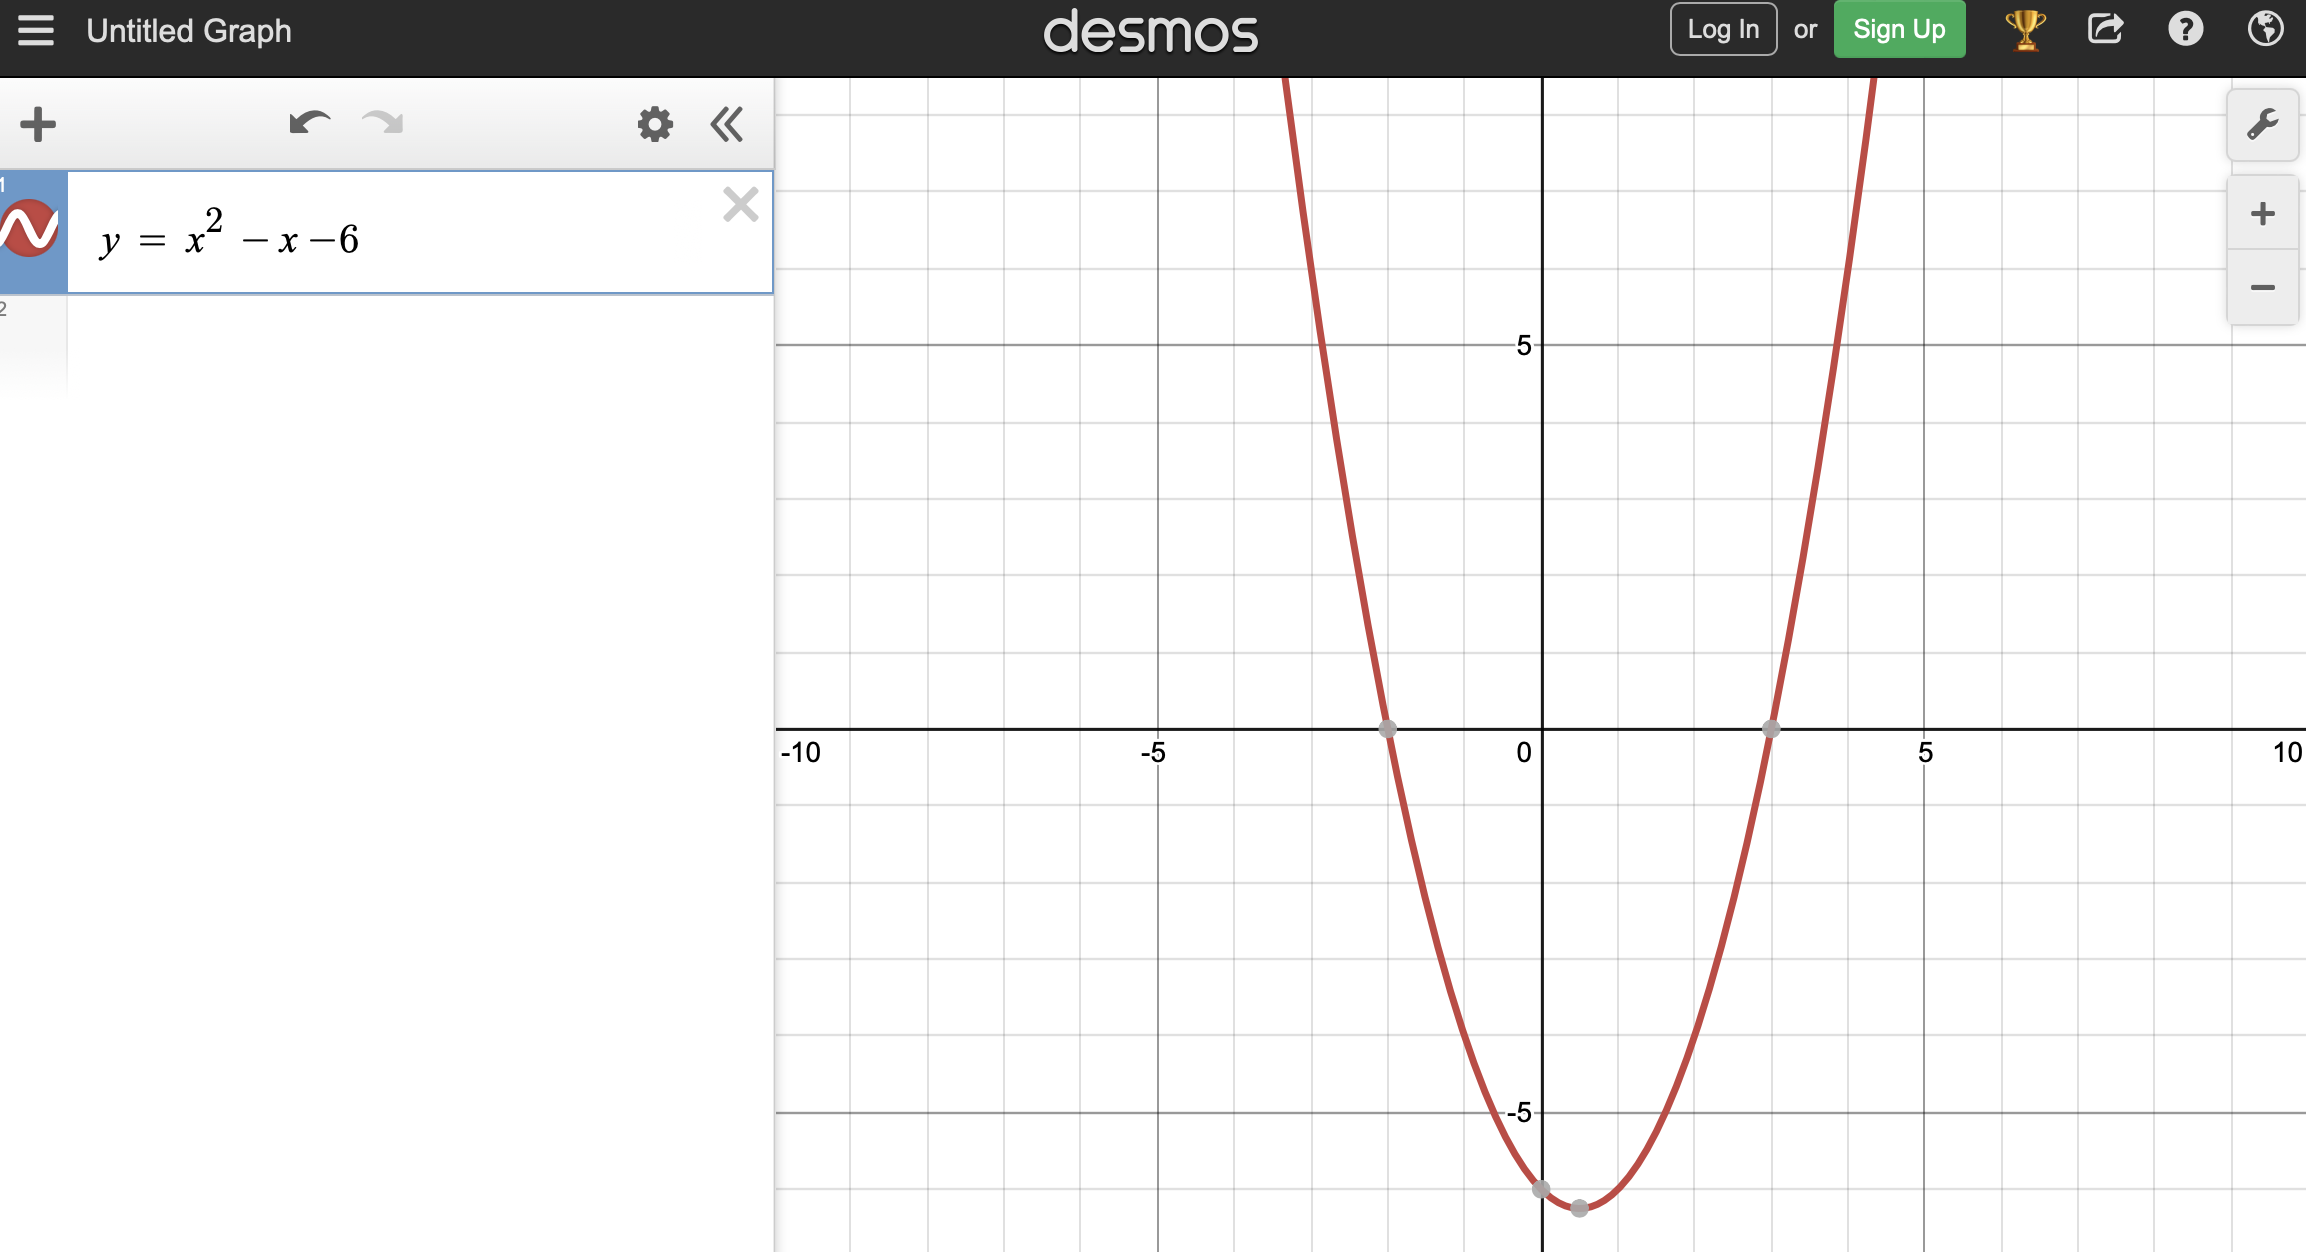
\includegraphics[width=0.85\textwidth]{Desmos.png}

\section{Even and Odd Functions}


\subsection{Even Functions}

An even function is symmetric about the y-axis. That means if you fold the graph along the y-axis, both sides will match perfectly. Note that the input value yields the same output regardless of whether the input value is positive or negative. 


\begin{mdframed}[style=important, frametitle={Even Functions}]

A function \( f(x) \) is even if  
\[
f(-x) = f(x)
\]  
for all \( x \) in its domain.
\end{mdframed}
Examples:
\begin{itemize}
  \item \( f(x) = x^2 \)  
  \item \( f(x) = \cos(x) \)  
  \item any \( f(x) = x^n \) where \( n \) is an even number
  \item \( f(x) = |x| \)
\end{itemize}

On a graph, a function will be a mirror image across the y-axis.

\subsection{Odd Functions}

An odd function is symmetric about the origin. That means if you rotate the graph $180^\circ$ about the origin, it lands on itself. Algebraically, when you input a value $k$, you get some output $n$; if you negate that input as $-k$, the output is also negated resulting in $-n$.


\begin{mdframed}[style=important, frametitle={Odd Functions}]

A function \( f(x) \) is odd if  
\[
f(-x) = -f(x)
\]
for all \( x \) in its domain.

Equivallently, 

\[ f(x) + f(-x) = 0 \]
for all \( x \) in its domain.
\end{mdframed}

\begin{itemize}

  \item \( f(x) = x^3 \)  
  \item \( f(x) = \sin(x) \)  
  \item \( f(x) = \tan(x) \)  
  \item any \( f(x) = x^n \) where \( n \) is an odd number
\end{itemize} 

On a graph, rotating the graph $180^\circ$ about the origin will yield the same graph.
\subsection{Neither Even Nor Odd}
Some functions are neither even nor odd. 

For example, \( f(x) = x^3 + 1 \) does not satisfy either condition.
% FIXME do we need to talk about end behavior, limits, symetry, etc
%%%%%%%%%%%%%%%%%%%%%%%%%%%%%%%%%
%% Bookfooter.tex by Aaron Hillegass
%% Nov 8, 2020

\appendix

\chapter{Answers to Exercises}
\shipoutAnswer

\bibliography{references}

\printindex

\end{document}